%%%%%%%%%%%%%%%%%%%%%%%%%%
% MSc Project Background Report Template
% Prof. Roger K. Moore
% University of Sheffield
% 22 March 2017
%%%%%%%%%%%%%%%%%%%%%%%%%%


\documentclass[11pt,oneside]{book}
\usepackage{url}
\usepackage[margin=1.2in]{geometry}
\usepackage{setspace}
\usepackage{amsmath}
\usepackage[toc,page]{appendix}
\usepackage[none]{hyphenat} % turn hyphenation off by default
\usepackage{graphicx}
\usepackage[parfill]{parskip}
\usepackage{float}
\usepackage{pgfplots}
\restylefloat{table}
\usepackage{array}
\usepackage{tcolorbox}
\usepackage{hyperref}
\usepackage{nameref}
\usepackage{rotating}
\usepackage{pgfplots}
\usepackage{tikzsymbols}
\usepackage{multirow}
\usepackage{amssymb}
\usepackage{fontspec}
\usepackage{xcolor}
\usepackage{soul}
\newfontfamily\DejaSans{DejaVu Sans}
\usepackage{graphicx}% http://ctan.org/pkg/graphicx

\DeclareMathOperator*{\argmax}{arg\,max}  % in your preamble
\DeclareMathOperator*{\argmin}{arg\,min}  % in your preamble 

\begin{document}


\begin{titlepage}

% You need to edit the details here

\begin{center}
{\LARGE University of Sheffield}\\[1.5cm]
\linespread{1.2}\huge {\bfseries William Briggs 12 Month Report}\\[1.5cm]
\linespread{1}

\includegraphics[width=5cm]{images/tuoslogo.png}\\[1cm]
{\Large William Briggs}\\[1cm]
{\large \emph{Supervisor:} Dr Mark Stevenson}\\[1cm]
{\large \emph{Panel:} Professor Lucia Specia, Professor Richard Clayton}\\[1cm]
Department of Computer Science\\[2cm]
\today
\end{center}

\end{titlepage}

% -------------------------------------------------------------------
% Declaration
% -------------------------------------------------------------------


% -------------------------------------------------------------------
% Abstract
% -------------------------------------------------------------------

\chapter*{\Large \center Abstract}

Medical data comes in large volumes, making it a challenge for systematic reviewers to process and find relevant information. Being able to apply automatic techniques to this field presents itself as a suitable application for natural language processing. As part of this report two areas were examined as potential candidates for future work. We critically evaluated existing methods to finding stopping points in ranked document collections as well as proposing some new methods. As part of the CLEF 2018 task for technology assisted reviews we built an IR system that uses limited information for retrieving relevant documents for a systematic review.
 


% -------------------------------------------------------------------
% TOC etc
% -------------------------------------------------------------------

\tableofcontents
\listoffigures
\listoftables

\setstretch{1.1} 

\mainmatter

\chapter{Introduction} \label{intro}

Medical literature poses interesting challenges for Natural Language Processing (NLP) researchers. The sheer volume of medical data makes it difficult for humans to process efficiently.

Evidence-based medicine has become an important aspect of health care and policy making. One key task is the creation of systematic reviews. Systematic reviews are transparent reviews that aim to pull together and critically analyse and summarise relevant literature to a topical question \cite{Gough2012}. The process of creating a systematic review is rigorous and time consuming with varying degrees of complexity in-between steps \cite{O’Mara-Eves2015}. This report will look at the existing  work done using NLP as part of the systematic review process as well as the novel work done by myself so far.

We first review the stages involved in creating a systematic review \ref{stepssr}. We break the steps down by looking at the PICO strategy \cite{pico}. By breaking the steps down, it becomes easier to examine potential candidates for applying NLP techniques to the process. Areas for research are then identified.

We then move on to look at stopping methods for systematic reviews. \ref{stops} Stopping methods are about finding a suitable stopping point given a list of ranked documents. Two existing methods are examined; the target method and the knee method. 

In the next section we identify some relevant research questions within the field \ref{rq}. Three areas are focused on: Automated Decision Making of Relevant Studies \ref{dm}, Information Extraction From Studies \ref{ie} and Stopping Methods 

The work completed so far is then presented \ref{novelw}. We look at using curves to make predictions of finding a stopping point, including using a Gaussian process. We then present our work for the automatic query generation process by using systematic review protocols as a basis for inferring the query.

Finally we look at future work \ref{fw}.



 \chapter{Literature Survey} \label{lit}

Systematic reviews have many different stages that propose themselves as a candidate for automation. This section is going to look at the techniques that have been applied for some of these stages in previous literature.

\section{Indexing and Querying Medline and Automated Query Generation}

Medline is a large collection of medical literature and data from around the world. Typically each entity will contain a title and an abstract containing some information on the study. Whilest Medline as a whole is very easy to access \cite{medline}, the large size and complexity of the data makes it difficult to retrieve the relevant information.

Being able to create a reliant index of Medline would help with the effectiveness of the queries. As such existing medline indexes and IR systems have been created \cite{nlm}.

\subsection{Automated Query Generation}

Being able to automate query generation for literature searching would save systematic reviewers a significant amount of time. However, medical literature queries are typically complex and contain multiple levels of logical operators and synonymous term look ups. This makes the task of creating a query manually in-its-self a challenging piece of work.

\subsubsection{Rapid Automatic Keyword Extraction Algorithm}

Rapid automatic keyword extraction (RAKE) is a keyword extraction algorithm was proposed by Rose, Engel and Cramer in 2010 \cite{rake}. This algorithm is used for taking the key pieces of information from text and is useful the domain of information extraction. This algorithm is of interest to us as it has potential usage within the field of query generation.

RAKE is heavily relies on stop-words and punctuation separators as an indicator for the importance of a phrases and words. RAKE will iterator over sequences of words until a stop-word or separator is found, this phrase/word is then split and extracted. Frequency of occurrence (tf) and word co-occurrence matrices can then be used to reduce the key-word set down further.

RAKE can be further optimized by specifying minimum term frequency rates to capture more prominent terms.


\section{Stopping Criteria} \label{stops}

Stopping criteria a topic of being able to know when to stop looking at a set of documents. This could be useful in a decision making process. Consider having 100 relevant documents, where each document contains a binary value. If we looked at 1/3 of these documents and saw a trend of positive values, we could use this to infer the reliability of the remaining documents.

Another use of stopping criteria is when filtering through potentially relevant documents. Consider a query that returns 10000 documents, of which only a small sub-set of these are relevant. Reviewers would need to filter through each of these 10000 documents to pull out the relevant ones. Or it could be that the reviewers are happy to hit a 90\% recall of relevant documents, and are happy to miss the remaining 10\% in exchange for time-saved.

Two key methods have been proposed for finding stopping points so far, the target method \cite{Satopa11} and the knee method. \cite{Cormack2016}. Both these methods are discussed below \ref{methods}



\subsection{Evaluation Metrics for Finding Stopping Points} \label{evalsstops}

In order to evaluate the suitability of our stopping method, we can use two evaluation metrics. The recall, which is simply the number of documents returned for a topic. The effort which is the number of documents we had to look at for a topic. 

\begin{equation}
Recall = \frac{R}{|D|}
\end{equation}

Where $R$ is the number of returned documents and $D$ is the set of relevant documents.

\begin{equation}
Effort = \frac{L}{|D|}
\end{equation}

Where $L$ is the number of returned documents looked at.

Naturally we could exclusively optimized each of the parameters by either returning everything in the document collection ($R$ = $|D|$) or by just looking at a single document. ($L$ = 1)

Therefore it becomes difficult for us to evaluate our stopping criteria as we need to consider both of these parameters adjacently.

In response to this we can make use of two more evaluation metrics that tell use  more about the performance of our stopping method \cite{Cormack2016}

\begin{equation}
reliability = P [acceptable(S) == 1]
\end{equation}

reliability is computed over all searches and is read as the probability of the acceptability being 1. Where acceptability is calculated as:

\begin{equation}
  acceptability(S)=\begin{cases}
    1, & \text{$recall(S)>=0.7$}.\\
    0, & \text{$recall(S)<0.7$}.
  \end{cases}
\end{equation}

A stopping point is deemed to be acceptable if 70\% of the relevant documents have been found. As such, the reliability is an average over a search method.


\subsection{Existing Stopping Methods} \label{methods}

There are different approaches can be experimented with in finding an optimum stopping point.  Consider a percentage cut-off method, where we use the score similarity score for deciding if its worth continuing to look down the rankings:

\begin{equation}
	  Difference(D_i, D_i+1) > C
\end{equation}

Where difference returns a score of how close document $D_i$ and $D_i+1$ are together and $C$ is a cut-off constant. We can expand this to an example:

\begin{equation}
	  (1 -(0.73 / 0.75)) * 100 > 0.015
\end{equation}

Here we are saying if the two documents' scores are above 1.5\% then we should stop looking down the rankings.

We a basis of how stopping methods work, we can move on to more established and defined methods.


\subsubsection{Target}

The target method is a fairly straight forward approach to establishing a stopping point. It was first proposed by Cormack and Grossman \cite{Cormack2016}.

The target $T$ denotes how many documents we should randomly select from our initial query. A larger value of $T$ will increase the effort required as we are more likely to select a document towards the end of the query set. Documents are looked at until the target point $T$ has been reached.

While this approach is shown to acquire 95\% reliability, the effort needed is often significantly highly, often requiring us to look at huge volume of documents.

We can evaluate how well this method does against an existing set of relevance rankings. We will use the Sheffield run data from the CLEF 2017 task \cite{Kanoulas12017}. We found that a $T$ parameter of 5 was the lowest we could go to still acquire a reliability of over 70\%. Overall we were able to obtain an average recall of 90\% by making an average effort of 58\%.

\subsubsection{Knee Method}






  \chapter{Research Questions} \label{rq}

In this chapter we will present some possible research areas for systematic reviews.

\section{Automated Decision Making of Relevant Studies} \label{dm}

Once relevant studies have been identified by their abstracts, reviewers are required to process the studies and extract useful information for the systematic review. Many of these studies will not be useful and can be discarded, but not without the cost of the reviewer having to look at the content.

A useful piece of research would be to determine if a study is relevant to the systematic review question. 

There are two potential routes that could be taken for the investigating this task. The first approach would be to use existing information from the systematic review (ie the protocol) and determine if the study contains the information. A second approach would be to a semi-supervised learning method, having the reviewer look at a subset of the studies, so we can then build a classifier for the remaining studies. Both of these approaches can be applied to the abstract screening and the data filtering stage of the systematic review. For the abstract screening we would be trying to predict if a study is relevant, by looking at the abstract. For the data filtering stage we would be looking at the actual text of the study (typically a pdf file)

There are many challenges for this research topic. Not all studies are publicly available and are often protected by publishing licences. This makes it difficult to gather data. Another challenge is having to deal with such a broad range of data, as well as the pdf format studies.

\section{Information Extraction From Studies} \label{ie}

In a similar vein to the first topic \ref{dm} we could also look at extracting the relevant information from a study. Often empirical data is identified in studies and extracted to generate a tree diagram:

\begin{figure}[H]
\center
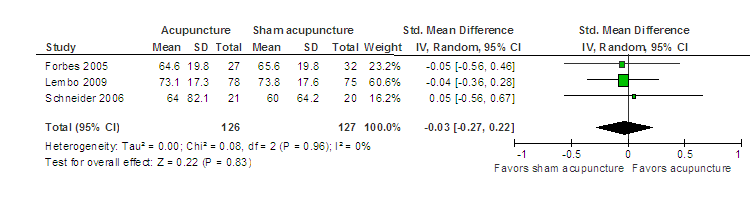
\includegraphics[width=16cm]{figures/tree.png}
\caption{Tree diagram example, all credit for diagram goes here \cite{Manheimer2012}}
\end{figure}

These tree diagrams contain summarized information from the relevant studies. Studies that contain more useful (i.e higher number of participants) have smaller confidence margins and vice-versa for smaller studies.

An interesting area of research would be identifying empirical data in a study to generate these tree diagrams automatically.

The challenge in this task is gathering training data that is sufficiently marked as to where key information occurs within a study. This would would also still involve working with a limited number of studies and pdf documents.



 \chapter{Novel Work} \label{novelw}

In this section the work completed so far will be presented. 

We first look at the CLEF 2017 runs, these are the datasets we will use for applying and evaluating our stopping methods. We establish a baseline result (Oracle); this tells use the best performance we could possibly get for each run. We then move on to evaluate two new methods that we developed to stopping, a percentage cut-off and a similarity score cut-off approach.

Further work looks at a different approach to stopping using partition sampling. We use a portion of the document collection to observe the distribution of the data and then predict the remaining portion. We first apply a curve to our data and then move on to use a Poisson Process.

Finally we look at an idea for building upon the dataset we are using by extracting more information from a study's full text. We present some initial findings as to how possible it is to retrieve these texts through automated techniques.



\section{CLEF 2017 Runs} \label{clefRuns}

For the CLEF 2017 Technologically Assisted Reviews in Empirical Medicine \cite{Kanoulas12017}, participants were expected to submit runs for ranking documents. Participants were given complex boolean queries that could be used for extracting relevant information to rank the documents. These runs were later released for public access \footnote{https://github.com/CLEF-TAR/tar/tree/master/2017-TAR/participant-runs}

\begin{table}[!htbp]
\scalebox{0.75}{
\centering
\caption{The 6 runs sampled from the CLEF 2017 task.}
\label{my-label}
\begin{tabular}{|l|l|l|}
\hline
Run                  & Description                                                                    & Reference                                     \\ \hline
Sheffield-run-2      & Sheffield-2 used tfidf similarity along with standard pre-processing           & \cite{Alharbi2017}           \\ \hline
Waterloo A-rank-cost & Waterloo used a baseline model implementation from the TREC Total Recall Track & \cite{cormack2017technology} \\ \hline
Waterloo B-rank-cost & -                                                                              & \cite{cormack2017technology} \\ \hline
auth run-1           & AUTH used a learning-to-rank approach and used both batch and active learning  & \cite{Anagnostou2017clef}    \\ \hline
auth run 2           & -                                                                              & \cite{Anagnostou2017clef}    \\ \hline
ntu run-1            & Used convolutional neural networks (CNN)                                       & \cite{lee2017clef}           \\ \hline
ucl full-text        & Used a deep learning model architecture                                        & \cite{singh2017identifying}  \\ \hline
\end{tabular}
}
\end{table}


We have taken 6 ranking sets of which are of different quality. The Waterloo and AUTH ranks are the best rankings followed by Sheffield. The UCL and NTU submissions feature poorer quality rankings. We tried to take runs that had a varying level of quality in the rankings.

CLEF 2017 runs will follow a format similar to the example below. The most important information being the topic id and the document id. 


\begin{tcolorbox} \label{scoreExample}
CD010775 NF 19307324 1 0.27152011529138564 Test-Data-Sheffield-run-2 
\end{tcolorbox}

Results can be evaluate using qrel files, supplied as part of the CLEF 2017 data. These files contain relevant documents for each topic, and are formatted as follows:

\begin{tcolorbox}
CD008803     0  21467181     0  \\
CD008803     0  20872357     1  \\
CD008803     0  23837966     0 
\end{tcolorbox}

Where the 1 or 0 on the right side indicates if the document is relevant for a study. Therefore the quality of the datasets can be observed by looking at how many of the relevant documents feature towards the top of the rankings.


\section{Baseline Approaches to Stopping} \label{baselineapp}

We can now establish some baseline approaches for finding stopping points. Approaches are heavily dependent on the initial rankings of the document collection, and naturally assume more relevant documents feature towards the start of the collection. 

\subsection{Oracle Scores} \label{oracleScores}

Looking at the oracle scores for each set of rankings will tell us the best we can possibly for do this task.  We will used the 70\% recall benchmark.

These scores are calculated as the minimum amount of effort that could be made to achieve 70\% recall. We first loop over each topic and update a count each time a relevant document is found. We then examine the recall each time the count is updated and determine if the threshold score has been reached (70\%). If 70\% has been reached we stop iterating over the rankings and calculate the effort made up to this point.

Results are taken as averages over all topics.

\begin{table}[H]

\centering
\begin{tabular}{|c|c|c|c|c|} 
\hline
 Submission & recall & reliability & effort  \\ 
 Test\_Data\_Sheffield-run-2 & 0.7 &	1.0	&	0.11 \\ 
 Waterloo A-rank-cost & 0.7 &	1.0	&	0.07 \\ 
 Waterloo B-rank-cost & 0.7 &	1.0	&	0.06 \\ 
 auth run-1 & 0.7 &	1.0	&	0.08 \\ 
 auth run-2 & 0.7 &	1.0	&	0.09 \\ 
 ntu run-1 & 0.7 &	1.0	&	0.4 \\ 
 ucl full-text & 0.7 &	1.0	&	0.67 \\ 
 \hline
\end{tabular}

\caption{Lowest effort possible to find 70\% of relevant documents. }

\end{table}

These scores highlight the importance of the ranking methods for finding a stopping point. The best performer, Waterloo B-rank-cost needs just 6\% effort to hit 100\% reliability. The worst performer, ucl full-text requires 67\% effort for the same level of reliability.


\subsection{Percentage cut-off method} \label{perCutOffMethod}

As a first approach we could simply take a cut of the document collection and evaluate how many relevant documents we have retrieved. This likely to be very dependant on the initial rankings of the document collection. 

\begin{table}[!htbp]
\scalebox{0.75}{
\centering
\caption{Comparison of results between rankings when looking at a percentage of the ranked documents.}
\label{my-label}
\begin{tabular}{|l|l|l|l|l|l|l|l|l|l|l|l|l|l|l|l|}
\hline
\% of Documents      & \multicolumn{3}{l|}{10\%}     & \multicolumn{3}{l|}{25\%} & \multicolumn{3}{l|}{50\%} & \multicolumn{3}{l|}{75\%} & \multicolumn{3}{l|}{90\%} \\ \hline
Run                  & Recall & Reliability & Effort & -       & -      & -      & -       & -      & -      & -       & -      & -      & -       & -      & -      \\ \hline
Sheffield-run-2      & 0.49   & 0.16        & 0.10   & 0.74    & 0.66   & 0.25   & 0.91    & 0.93   & 0.50   & 0.98    & 1.00   & 0.75   & 0.99    & 1.00   & 0.90   \\ \hline
Waterloo A-rank-cost & 0.80   & 0.6         & 0.10   & 0.91    & 0.93   & 0.25   & 0.98    & 1.00   & 0.50   & 0.99    & 1.00   & 0.75   & 0.99    & 1.00   & 0.90   \\ \hline
Waterloo B-rank-cost & 0.73   & 0.63        & 0.10   & 0.90    & 0.93   & 0.25   & 0.98    & 1.00   & 0.50   & 0.99    & 1.00   & 0.75   & 0.99    & 1.00   & 0.90   \\ \hline
auth run-1           & 0.72   & 0.63        & 0.10   & 0.90    & 0.93   & 0.25   & 0.97    & 1.00   & 0.50   & 0.99    & 1.00   & 0.75   & 0.99    & 1.00   & 0.90   \\ \hline
auth run 2           & 0.68   & 0.60        & 0.10   & 0.88    & 0.9    & 0.25   & 0.97    & 1.00   & 0.50   & 0.99    & 1.00   & 0.75   & 0.99    & 1.00   & 0.90   \\ \hline
ntu run-1            & 0.19   & 0.00        & 0.10   & 0.39    & 0.06   & 0.25   & 0.62    & 0.43   & 0.50   & 0.83    & 0.83   & 0.75   & 0.91    & 0.93   & 0.90   \\ \hline
ucl full-text        & 0.08   & 0.00        & 0.10   & 0.22    & 0.00   & 0.25   & 0.46    & 0.03   & 0.50   & 0.70    & 0.70   & 0.75   & 0.87    & 0.93   & 0.90   \\ \hline
\end{tabular}
}
\end{table}

All scores are averaged over the entire ranking set.

Sheffield has an average recall of 0.49 by the time 10\% of the documents have been observed. Waterloo has achieved 80\% recall by this point. After looking through 25\% of the rankings Waterloo and AUTH have achieved around 90\% recall of documents.

The limitation of this approach is the effort required looking through documents is still high. We want to lower this effort as much as possible, whilst only having to observe relevant documents.


\subsection{Similarity score cut-off method} \label{simScoreMethod}

A similarity score method will assume each document in the rankings has a score associated with it. Consider the ranking format described in \ref{clefRuns}. The 5th column describes a similarity between the document and the query. Similarity scores gradually decline as we descend down the rankings.


For the Sheffield set of rankings, the similarity score comes from the cosine similarity between a vectorized query and document. 

The similarity score can be used derive a stopping point. This method works by looking at documents $D_i$ and $D_{i+1}$ and determining if the difference between the similarity scores has become too large. This method will work on the basis that documents that are no longer relevant will have a sudden drop in score such that we can identify this as our stopping point.

\begin{equation}
	  Difference(D_i, D_{i+1}) > C
\end{equation}

Where difference returns a score of how close document $D_i$ and $D_{i+1}$ are together and $C$ is a cut-off constant. We can expand this to an example:

\begin{equation}
	  (1 -(0.73 / 0.75)) * 100 > 0.015
\end{equation}

Here we are saying if the two documents' scores are above 1.5\% then we should stop looking down the rankings.


\begin{table}[H]
\centering
\begin{tabular}{|c|c|c|c|c|} 
\hline
 $dif(D_i, D_{i+1})$ & recall & reliability & effort  \\ 
 0.01\% & 0.025 &	0.000	&	0.0023 \\ 
 0.05\% & 0.120 &	0.100	&	0.100 \\ 
 1\% & 0.359 &	0.333	&	0.333 \\ 
 2\% & 0.880 &	0.860	&	0.860 \\ 
 5\% & 1.000 &	1.000	&	1.0000 \\ 
 \hline
\end{tabular}

\caption{Similarity cut-off comparison for stopping for Test\_Data\_Sheffield-run-2. Using cosine similarity scores.}
\end{table}

These results are highly sensitive to the similarity score and show it is difficult to use this score as an effective measure for stopping. We found similarity scores rarely have sudden drops in values, making it difficult to use this method to identify a stopping point.

As an alternative approach, we can look at just the top document $D_1$, and compare it to the succeeding documents $D_{1+i}$ in the rankings. We can formulate this as follows:

\begin{equation}
	  Difference(D_1, D_{1 + i}) > C
\end{equation}

\begin{table}[H]
\centering
\begin{tabular}{|c|c|c|c|c|} 
\hline
 $dif(D_1, D_{1+i})$ & recall & reliability & effort  \\ 
 10\% & 0.048 &	0.000	&	0.004 \\ 
 20\% & 0.063 &	0.000	&	0.007 \\ 
 30\% & 0.113 &	0.000	&	0.152 \\ 
 40\% & 0.191 &	0.030	&	0.029 \\ 
 50\% & 0.319 &	0.060	&	0.063 \\
 60\% & 0.460 &	0.200	&	0.113 \\ 
 70\% & 0.638 &	0.433	&	0.210 \\ 
 80\% & 0.841 &	0.800	&	0.387 \\ 
 90\% & 0.979 &	1.000	&	0.679 \\ 
 100\% &1.000 &	1.000	&	1.000 \\  
 \textbf{85.5\%} & \textbf{0.934} &	\textbf{1.000}	&	\textbf{0.538} \\  
 \hline
\end{tabular}

\caption{Similarity cut-off comparison for stopping for Test\_Data\_Sheffield-run-2. Using cosine similarity scores. Compares first document to succeeding documents}
\end{table}

We found results to be much better when using the first document to look for a stopping point. 85.5\% difference in first and subsequent documents was found to be the point for hitting 1.0 reliability. This comes at the expense of making just over 50\% effort.

\section{Sample Methods to Stopping} \label{samplemethods}

The limitations of the methods presented in \ref{baselineapp} is that they they still require looking through a large volume of documents.

The approaches in this section will use sampling methods. These approaches assumes we have sensible ranking algorithm for returning documents for a query. They work by generating a sample set, which acts as our model for predicting a stopping point. Therefore the quality of these methods will depend on the sparseness of the document rankings, making it challenging to establish a single stand-out method.

The first step for these methods is to generate a sample set. We used an interval method for generating our set, i.e select every $N$th document. The intuition being that the distribution of relevant document in the sample set, should be similar to that of the complete set of relevant documents. This makes it suitable to use as a model. 


\iffalse
A limitation of this sampling method is that for topics with very few documents it is easy for a sample to miss many of them. This creates a subset set bias, where one set contains a larger percentage of relevant documents. Consider a query that returns 10000 candidate documents of which only 10 have been pre-determined to be relevant. Its not too unlikely that a randomly sampled subset would contain 0 relevant documents. We can use the following equation to tell us how much information we can take from a pre-evaluated topic:

\begin{equation}
I = \frac{rel(T_i)}{|T_i|}
\end{equation}

Where $T_i$ is a given topic and $rel$ computes the number of relevant documents for that topic. Therefore $I$ is telling us how useful the topic is at fitting a curve. We can take the average simply by taking the mean of $I$ across all topics:

\begin{equation}
Usefullness = \frac{\sum{I}}{|T|}
\end{equation}
\fi


\subsection{Curve Fitting}

Our first approach is to fit a non-linear curve against a sample set. We used a sample size of 3. We opted for an exponential curve as the number of relevant documents found will increase as more documents are looked, but eventually level out as relevant documents become less frequent.  

\begin{equation}
F(x) = n - ae^{-kx}
\end{equation}

Where $a$, $k$ and $n$ are learnt weights and $x$ is an associated return rate for a document. We generate the curve using the non-linear least squares algorithm \cite{leastsqures}. 


\iffalse
We can visualise the curve along with the confidence intervals. The Y axis is the predicted number of relevant documents for the topic. X axis shows the true number of documents returned for the query. 

\begin{figure}[H]
\center
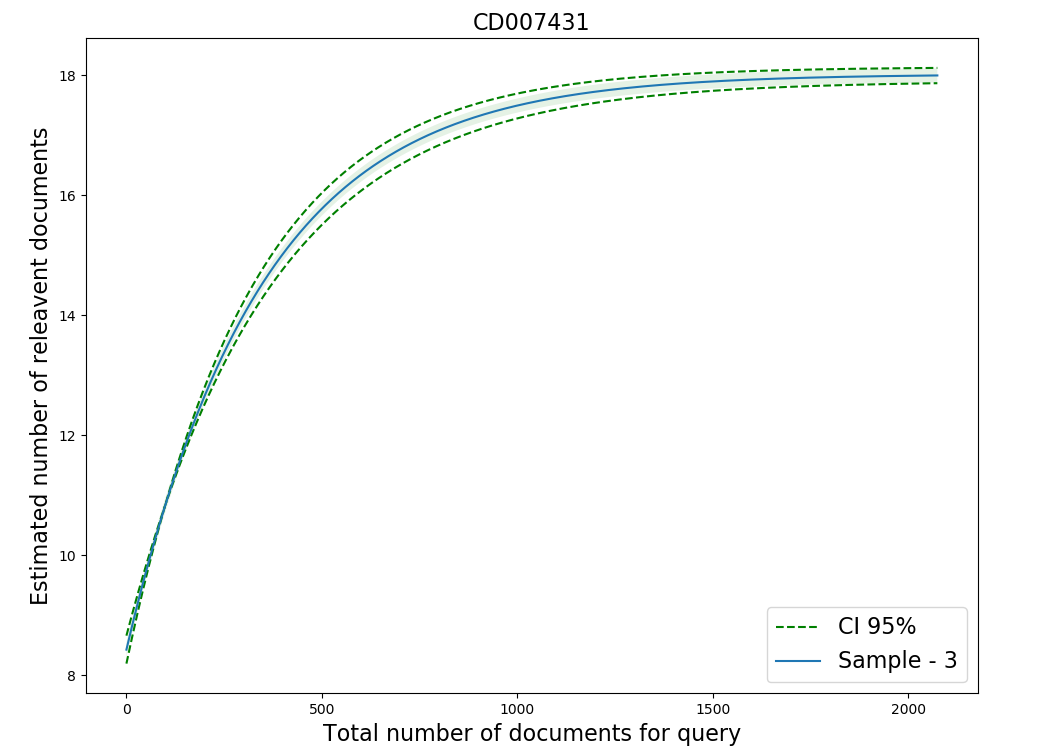
\includegraphics[width=10cm]{figures/curve_fit_example.png}
\caption{Example of fitting a curve for a topic using sampling}
\end{figure}

\begin{table}[H]
\centering
\begin{tabular}{|c|c|c|c|} 

 \hline
 sample size & recall & reliability & effort  \\ 
 1 & 0.91 &	0.96	&	1 \\ 
 3 & 0.66 & 0.5	&	0.48 \\ 
 5 & 0.481 & 0.33	&	0.315 \\ 
 \hline
\end{tabular}
\caption{Comparison of different sample intervals against recall and effort. Ranking Method: Test\_Data\_Sheffield-run-2 \cite{Alharbi2017}}

\end{table}

\fi


\subsubsection{Curve Predictions}

\iffalse
\begin{table}[H]
\centering
\begin{tabular}{|c|c|c|c|c|} 

 \hline
 Submission & recall & reliability & effort & topics sampled  \\ 
 Test\_Data\_Sheffield-run-2 & 0.68 &	0.53	&	0.50 & 30 \\ 
 Waterloo A-rank-cost & 0.70 & 0.46	&	0.44 & 30 \\ 
 Waterloo B-rank-cost & 0.70 & 0.46	&	0.40 & 30 \\ 
 auth run-1 & 0.74 & 0.53	&	0.43 & 30 \\ 
 auth run-2 & 0.70 & 0.50	&	0.43 & 30 \\ 
 ntu run-1 & 0.71 & 0.43	&	0.68 & 30 \\ 
 ucl full-text & 0.86 & 0.8	&	0.91 & 30 \\ 
 \hline
\end{tabular}
\caption{Evaluation of curve fitting for different CLEF 2017 runs. Sample size = 3. Results are taken as averages over all topics for search method. No topic cut-off}

\end{table}
\fi


The number of topics was reduced down from 30 to 23 using a cut-off parameter. This reduces some of topics that contain fewer relevant documents and does not generate suitable prediction curves. We used a cut-off parameter of 0.5\%. This can be read as the proportion of relevant documents in a document collection must be atleast 0.5\%, which was found to be a suitable amount to give us a good volume of topics.

We also include a confidence interval evaluation for lower bounded range of a $3\sigma$ confidence interval. The key advantages of using a curve as  method of evaluating stopping criteria is being able to make use of this confidence interval in a real systematic review. In the context of a systematic reviewers at the data filtering stage, we could specify that the system is 95\% certain that 70\% of relevant documents have been found. At which point the reviewer can decide if its worth continuing to look at documents.

\begin{figure}[H]
\center
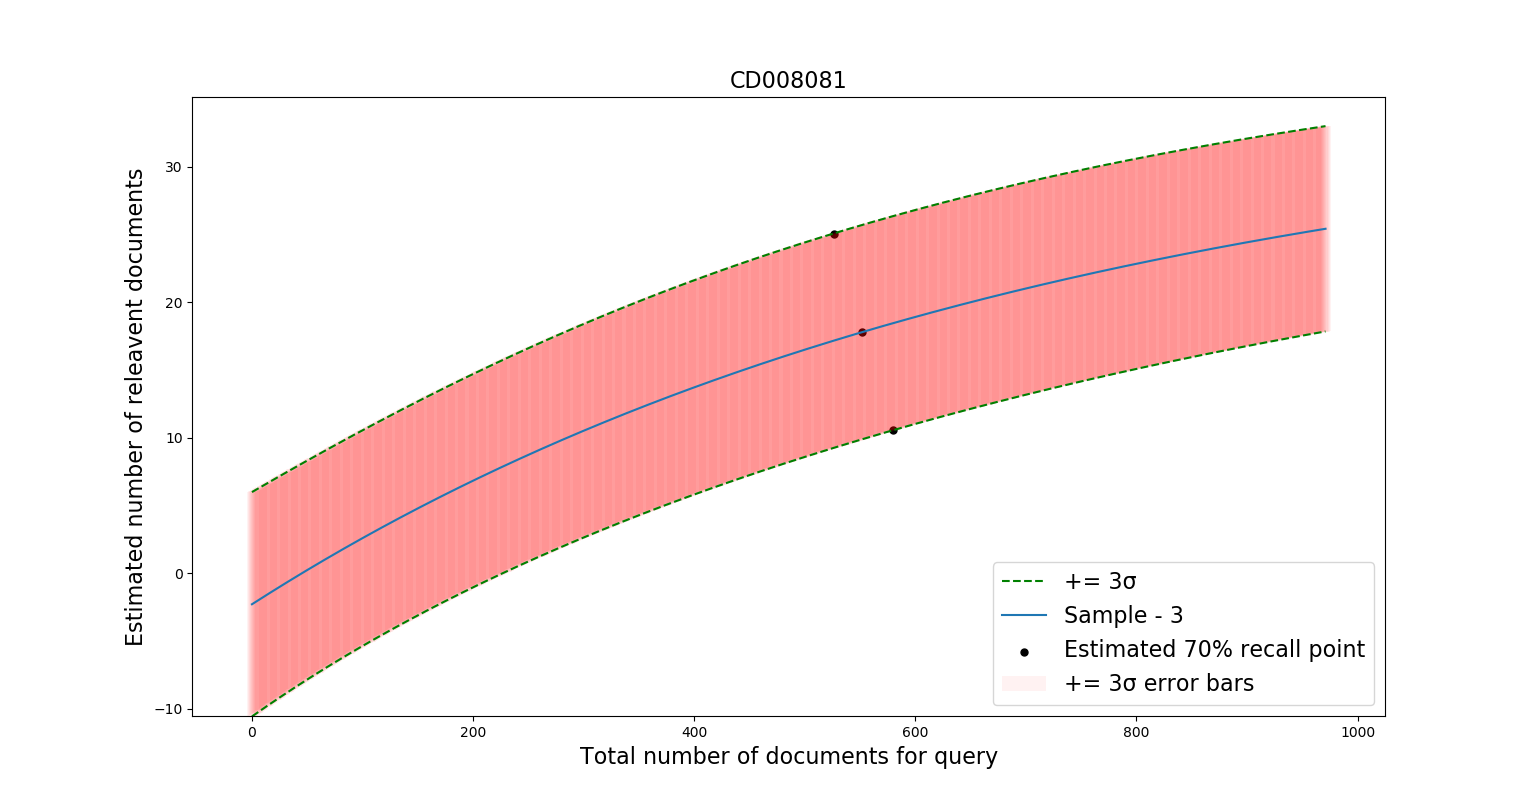
\includegraphics[width=17cm]{figures/cf_example.png}
\caption{Example of a prediction curve for topic CD008081. Confidence bars are included over $3\sigma$. Estimated point of hitting 70\% denoted by black point.}
\end{figure}

\begin{table}[H]
\scalebox{1}{
\centering
\begin{tabular}{|c|c|c|c|c|} 

 \hline
 Submission & recall-lower & reliability-lower & effort-lower & topics sampled  \\ 
 Test\_Data\_Sheffield-run-2 & 0.69 \, 0.74, &	0.52 \, 0.60	&	0.48 \, 0.51 & 23 \\ 
 Waterloo A-rank-cost & 0.71 \, 0.73, &	0.47 \, 0.47	&	0.43 \, 0.44 & 23 \\ 
 Waterloo B-rank-cost & 0.71 \, 0.75, &	0.52\, 0.82	&	0.41\, 0.43 & 23 \\ 
 auth run-1 & 0.72 \, 0.74, &	0.52 \, 0.60	&	0.41 \, 0.42 & 23 \\ 
 auth run-2 & 0.70 \, 0.72, &	0.52 \, 0.60	&	0.42 \, 0.43 & 23 \\ 
 ntu run-1 & 0.76 \, 0.74, &	0.56 \, 0.52	&	0.72 \, 0.70 & 23 \\ 
 ucl full-text & 0.86 \, 0.94, &	0.82 \, 0.86	&	0.91 \, 0.95 & 23 \\ 
 \hline
\end{tabular}
}
\caption{Evaluation of curve fitting for different CLEF 2017 runs. lower = lower-bound confidence interval. Sample size = 3. Results are taken as averages over all topics for search method. with 0.5\% cut-off}

\end{table}

We have deliberately compared two of the better participant rankings (Waterloo and auth) and two of the lower performers (ntu and ucl). We can see the quality of the initial rankings significantly influences the performance of our stopping criteria. This suggests there is a important relationship between using a curve to predict a stopping point and how good the initial ranking of documents is. 

Some of the datasets to produce curves due to the sparsity of relevant documents. In situations where this occurred, we returned everything for the given topic, resulting in 100\% recall at the expense of 100\% effort.

\iffalse
\subsection{Gaussian Process Fitting}

As an alternate approach to fitting a simple curve, we can apply a Gaussian Process (GP) \cite{ebden2008gaussian}. We will apply a constant kernel plus a squared-exponential kernel. GP was implemented using scikit learn classes. \footnote{http://scikit-learn.org/stable/modules/gaussian\_process.html}


\begin{table}[H]
\scalebox{1.0}{
\centering
\begin{tabular}{|c|c|c|c|c|} 

 \hline
 Submission & recall-lower & reliability-lower & effort-lower & topics sampled  \\ 
 Test\_Data\_Sheffield-run-2 & 0.73 \, 0.73, &	0.73 \, 0.73	&	0.50 \, 0.50 & 23 \\ 
 
 
 Waterloo A-rank-cost & 0.70 \, 0.70, &	0.40 \, 0.40	&	0.42 \, 0.42 & 23 \\ 
 
 
 Waterloo B-rank-cost & 0.73 \, 0.73, &	0.71 \, 0.71	&	0.41 \, 0.41 & 23 \\ 
 
 
 auth run-1 & 0.74 \, 0.75, &	0.56 \, 0.60	&	0.42 \, 0.42 & 23 \\ 
 
 
 auth run-2 & 0.72 \, 0.73, &	0.52 \, 0.52	&	0.42 \, 0.42 & 23 \\ 
 
 
 ntu run-1 & 0.67 \, 0.67, &	0.40 \, 0.40	&	0.64 \, 0.64 & 23 \\ 
 
 
 ucl full-text & 0.62 \, 0.62, &	0.52 \, 0.56	&	0.82 \, 0.82 & 23 \\ 
 \hline
\end{tabular}
}
\caption{Comparison of different of sample method using gp for different CLEF 2017 runs. lower = lower-bound confidence interval. Sample size = 3. Results are taken as averages over all topics for search method. with 0.5\% cut-off}

\end{table}


We found the GP is not truly representing the distribution of the data.

\begin{figure}[H]
\center
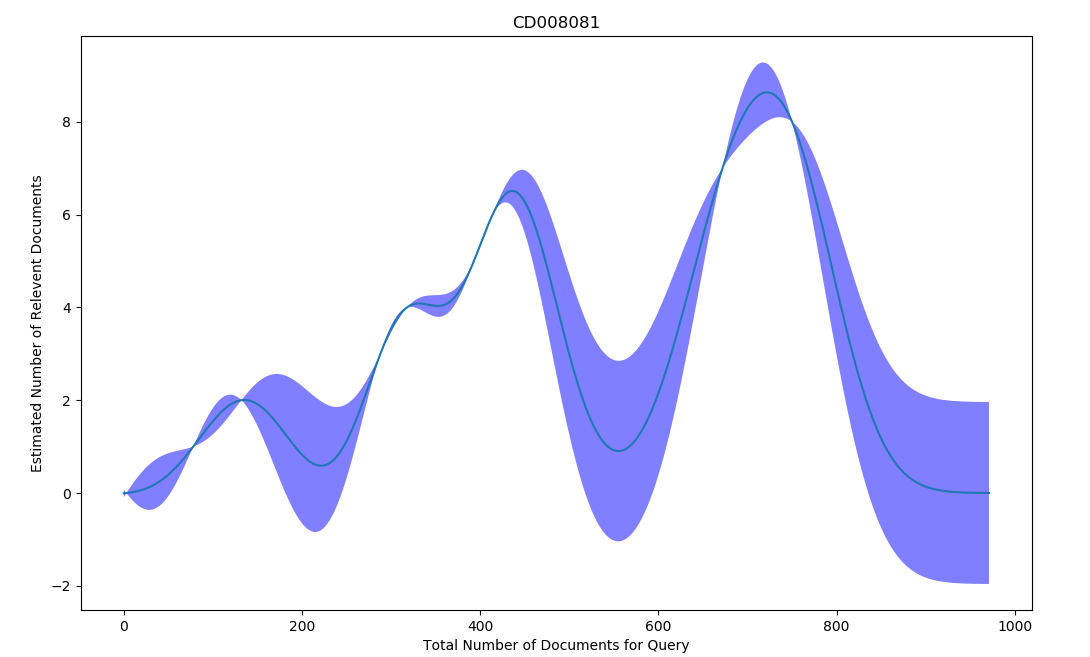
\includegraphics[width=12cm]{figures/GP_fit.png}
\caption{Visualisation of using a confidence interval for predicting a stopping point using a gp.}
\end{figure}


\subsection{Conclusion on Curve fitting and GP} \label{conclusCurveAndGp}

We implemented two methods for predicting stopping points in ranked medical studies. Our first approach used a general curve to estimate the point in which 70\% recall is likely to have been hit. Our second method used a Gaussian Process in the same way. We used a sampling method to generate our curves to makes predictions about the remaining studies.

\fi



\section{Poisson Process for Stopping Points} \label{window_samp}

A Poisson Process can be used to model points in time in which events occur. In this situation we wish to observe the rate in which a relevant document occurs in a collection of documents.

We can observe the relevant document distribution for each topic by plotting relevant document occurrences across the whole rankings.


\begin{figure}[H]
\center
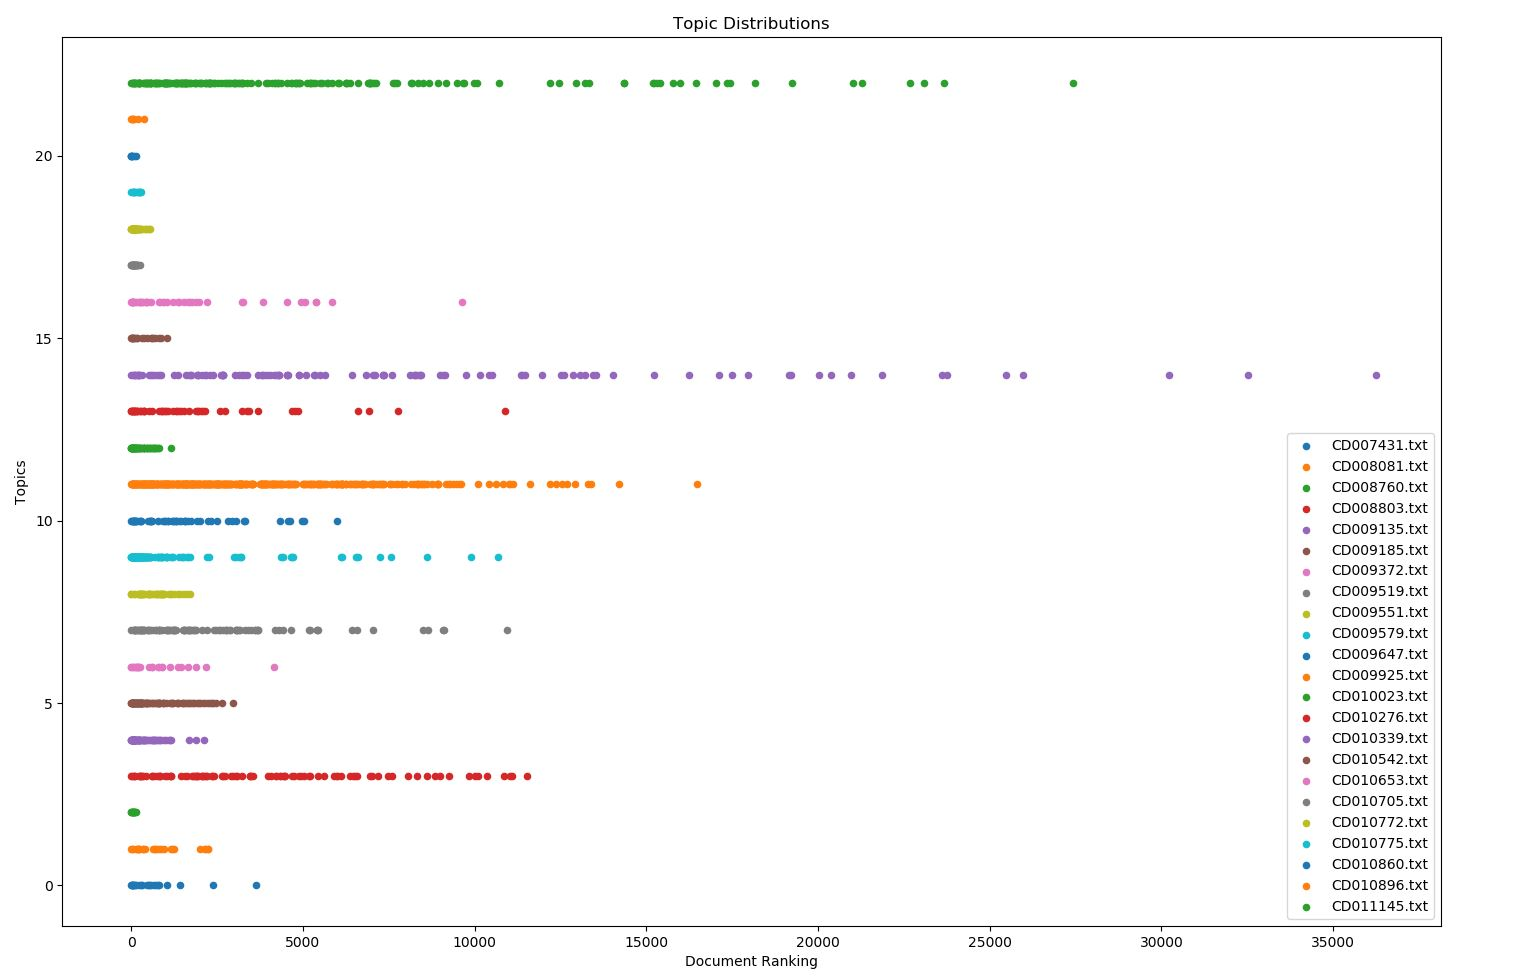
\includegraphics[width=15cm]{figures/distrib.jpg}
\caption{Relevant document distribution over Sheffield dataset}
\end{figure}

The quality of the initial rankings will determine how many relevant documents occur towards the start of the distribution. Naturally the number of relevant documents decrease as we proceed down the rankings.

The Poisson distribution is a way for us to model the occurrences of relevant documents in a fixed time-frame, in our situation, the number of documents returned by the query. To estimate the overall rate of which relevant documents occur, we can observe how many relevant documents occur within a threshold.


\begin{equation}
	  \lambda = \frac{r_i}{|D|}
\end{equation}

Where $r_i$ is the number of relevant documents in a sample set and $|D|$ is the number of documents in the sample set.

Supposing we sample 10\% of the 1000 documents, of which 7 relevant documents occur:

\begin{equation}
	  \lambda = \frac{7}{100} = 0.07
\end{equation}

We can use the rate parameter to estimate the probability of there being atleast one relevant documents, after observing $n$ documents:

\begin{equation}
	  P = 1 - e ^ {0.7n}
\end{equation}


\begin{figure}[H]
\center
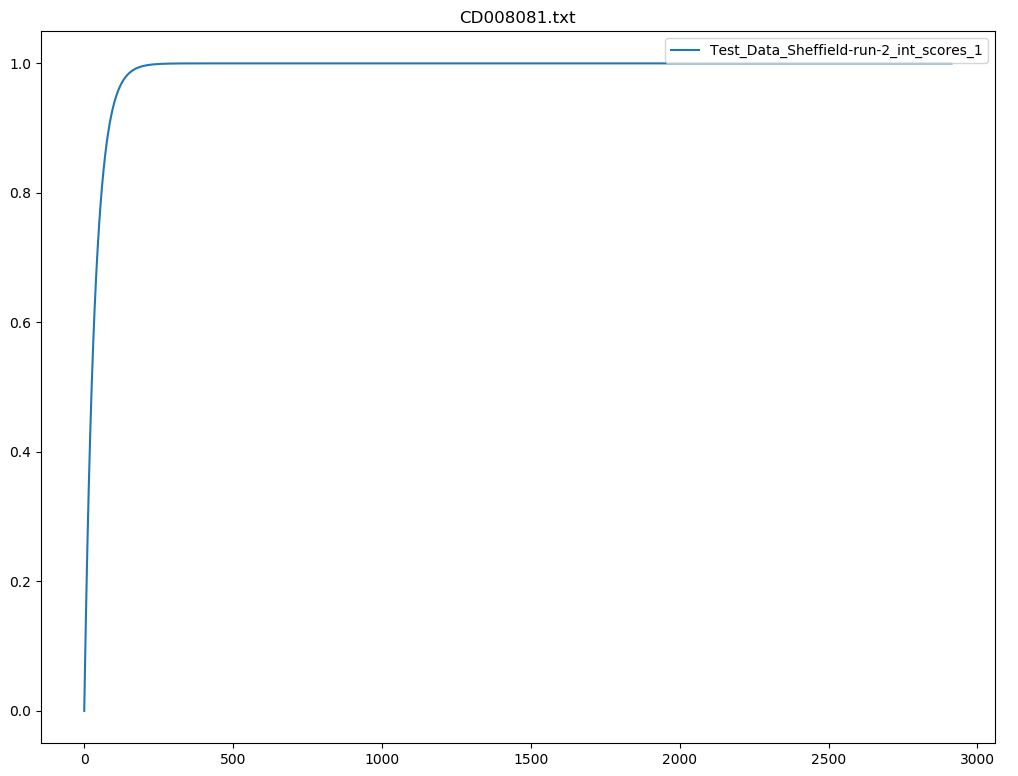
\includegraphics[width=10cm]{figures/probOneDoc.jpg}
\caption{Probability of seeing atleast one relevant document by sampling 10\% of documents for topic CD008081}
\end{figure}

The plot shows as we look at more documents, we are increasingly likely to have seen one relevant document. While this is useful to know, we can not use this as a method for predicting a suitable stopping point.

A Homogeneous Poisson process can be used to model the occurrences of relevant document and then used to predict the probability of there bring $r$ relevant documents after $n$ documents have been observed. 

\begin{equation}
	  P(r) = \frac{(\lambda n)^r}{r!} e ^ {-\lambda n}
\end{equation}


Due to the high likelihood that $r!$ will be exceeding large, we can use a stirling approximation, maintaining a similar value as to what we would have obtained computing the factorial.

\begin{equation}
	   r \approx \sqrt{2\pi r} \left( \frac{r}{e} \right) ^r
\end{equation}

By summing over the probability mass from for values of $n$ between 1 and the size of the document collection we can estimate at what point 95\% reliability (stopping point $s$) is reached. 

\begin{equation}
	   s = \sum_{0, i < 0.95}^{|n|} \frac{(\lambda i)^r}{stirling(r!)} e ^ {-\lambda i}
\end{equation}

The limitation of using an Homogeneous Poisson process is that the rate parameter is constant throughout distribution. This means if we looked at 10\% of the rankings the rate of relevant documents would be assumed to be constant for the remainder of the document collection. Therefore this method would only be suitable if we had a random relevance rate.


\begin{figure}[H]
\center
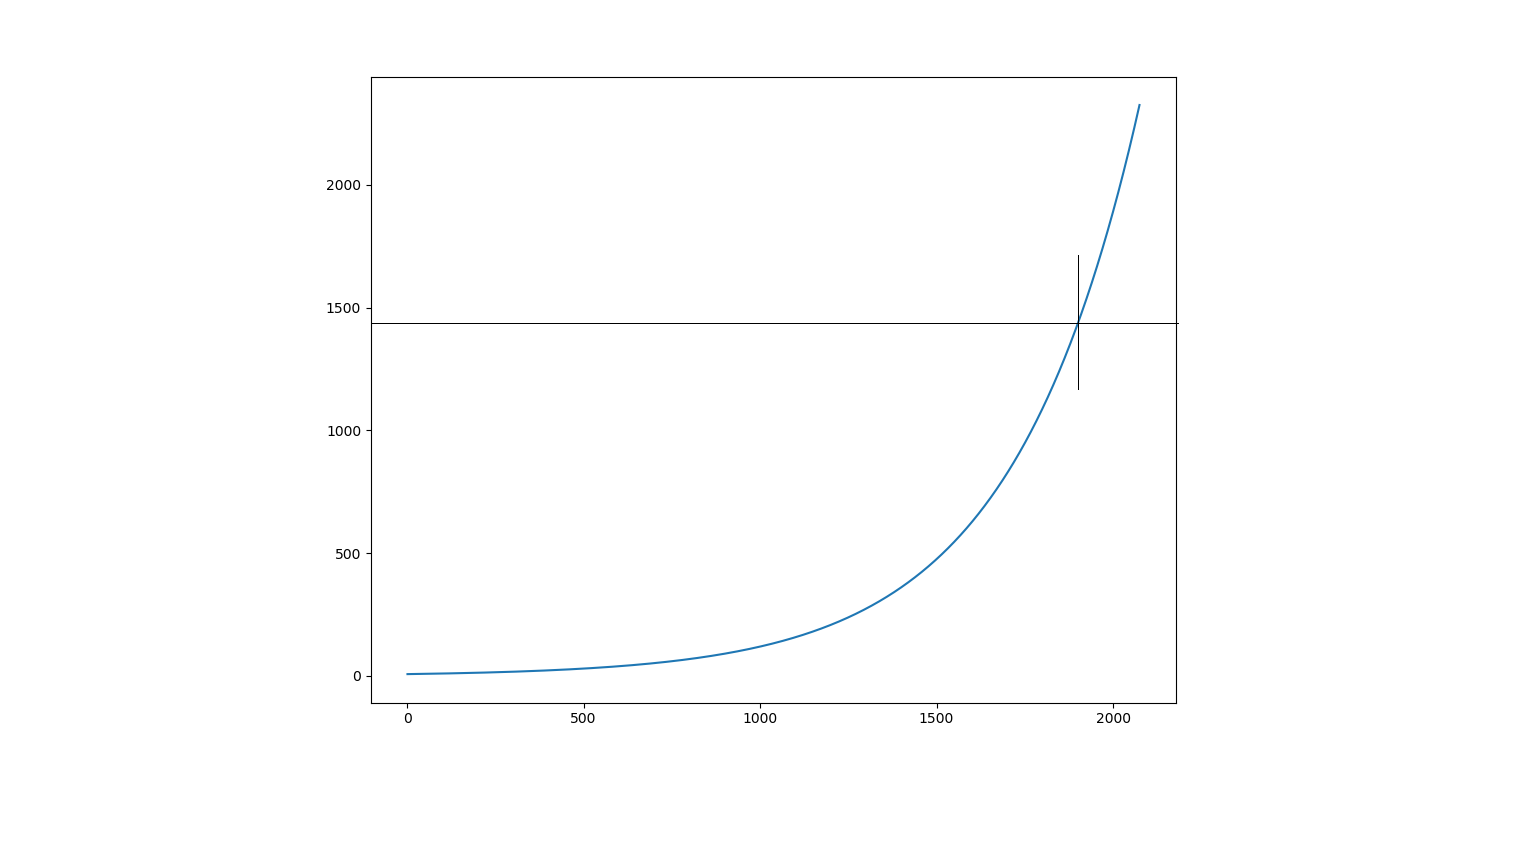
\includegraphics[width=16cm]{figures/overestimate.png}
\caption{Homogeneous Poisson process overestimating the rate of documents, resulting a prediction curve that would expect us to look at 1500 of the 2000 documents to reach 70\% recall}
\end{figure}

\subsection{Non-Homogeneous Poisson Process}

As the rate parameter is varies throughout the distribution of documents, we can use a Non-Homogeneous Poisson process. A Non-Homogeneous Poisson process is similar to an ordinary Poisson process, except that the average rate of arrivals is allowed to vary with time \cite{nonhomp}. 


\subsubsection{Non-Homogeneous Poisson Definition} \label{nn_pp_def}

We can use a non-homogenous poission process to estimate the number of relevant documents in a given interval by integrating the rate function $\lambda(x)$ across the interval.

We first define our intervals as $a$ and $b$ and integrate the values between them with respect to $x$

\begin{equation}
	   \int_a^b \lambda(x) d(x) = \Lambda(a, b)
\end{equation}

Therefore the probability of there being $r$ relevant documents in the interval $(a, b$)

\begin{equation}
	   P(N(a, b) = r) = \frac{[\Lambda(a,b)]^r}{r!} e^{-\Lambda(a,b)}
\end{equation}

We can make the assumption that the rate in which relevant documents appear is an exponential function.

\begin{equation}
	   \lambda(x) = ae^{kx}
\end{equation}

Therefore

\begin{equation}
	   \int \lambda(x) d(x) = \int ae^{kx} dx = \frac{a}{k}e^{kx}
\end{equation}

As we are only interested in knowing the total number of relevant documents, we assume that we are integrating from 0 to the total number of documents.

\begin{equation}
	   \Lambda(0, n) = \int_0^n ae^{kx}dx = \left[\frac{a}{k}e^{kx}\right]_0^n = \frac{a}{k}(e^{kn} - 1)
\end{equation}

So

\begin{equation}
	   P(N(0,n) = r) = \frac{(\Lambda(0,n))^r}{r!}e^{-\Lambda(0,n)} = \frac{\left(\frac{a}{k}(e^{kn} -1)\right)^r}{r!} e^{-(\frac{a}{k}(e^{kn} - 1)})
\end{equation}

Therefore given values for $a$ and $k$ which we can learn from fitting an exponential curve, we can predict the probability of there being $r$ relevant documents within the entire set of $n$ documents.


\subsubsection{Implementation Non-Homogeneous Poisson Process} \label{imp_non_hom}

\paragraph{Window Sampling} \label{window_samp}

It is useful for us to estimate the rate at which relevant documents occur. By iterating over each document in a returned set of documents, and evaluating the relevant documents in a given window, we can estimate this rate parameter. 

\begin{table}[H]

\centering
\begin{tabular}{|c|c|c|} 
\hline
 Document Rank & Relevant & RelScore  \\ 
 1 & Y &			1/3=0.33 \\ 
 2 & Y &			3/4=0.75 \\ 
 3 & N &			4/5=0.80 \\ 
 4 & Y &			3/5 =0.60 \\ 
 5 & Y &			2/5=0.40 \\ 
 6 & N &			2/5=0.40 \\ 
 7 & N &			1/4=0.25 \\
 8 & N &			0/3=0.00 \\
  
 \hline
\end{tabular}

\caption{Using window sampling with a window size of 2 either side.}

\end{table}

The challenge is being able to find an optimum sample size. A sample size that is too small will not provide enough information on the distribution of the surrounding documents. A sample size that is too large is a risk, as the if the documents rankings are sparse the rate estimations would not be as useful.

\paragraph{Poisson Process Steps} \label{pp_steps}

We created a Python-based implementation using scipy for the curve modelling. Our steps can be broken down as follows:

\begin{enumerate}
\item Load a run final into memory. For this task we used the Sheffield run data from CLEF 2017.

\item Create a frequency based distribution of the data for relevant documents, e.g 1, 1, 2, 3, 3, 3, 3, 4

\item Normalize the data for positions in which relevant documents occur e.g x = 1, 2, 3, 4, 5 y = 2, 12, 17, 34, 61

\item Use normalized data along with window sampling \ref{window_samp} to create a probabilistic relevant document frequency in a given window. 

\item Take a sample percentage from the distribution (start at 1\%). Use this percentage to fit an exponential curve ($ae^{kx}$) using non-linear least squares \footnote{\url{https://docs.scipy.org/doc/scipy/reference/generated/scipy.optimize.curve_fit.html}}. This provides values for $a$ and $k$ which can then be substituted into equation 4.16 to give the distribution of the total number of relevant documents.

\item Use weights from curve fit and Non-Homogeneous Poisson process to estimate the number of relevant documents across the entire collection. For values from $r: 0 \mapsto n$ we will get a probability of $r$ relevant documents. Assuming 95\% of documents is acceptable, we can sum over the probability mass until this value is reached.

\end{enumerate}

\paragraph{Finding an Optimum Window Size} \label{pp_steps}

To find a general window size for sampling we will observe the sum of the mean squared error over all topics for sampled data from 10\% to 40\%. We will consider sample window sizes in the range of 1 to 100.  This will tell us how well our exponential curve is fitting to the data for each window sample size.

\begin{figure}[H]
\center
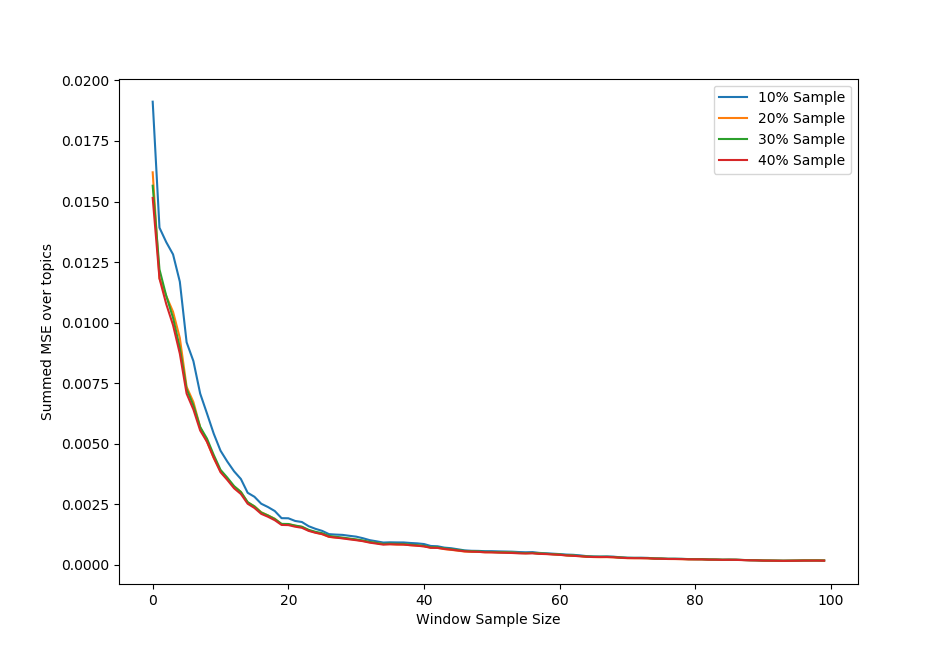
\includegraphics[width=15cm]{figures/sse_avg.png}
\caption{Comparison of different sample portions against sample window size}
\end{figure}

We can see a fairly steep drop decline between using a sample window of 1 to 20. As we reach 50, the curve has become almost flat. Therefore, we will use a sample window of 50 for the remainder of this work.


\paragraph{Results for Non-Homogeneous Poisson Process} \label{nn_pp_def}

Using the above definition and sample window we created a non-homogeneous Poisson process and generated some results. We still consider different sample portions for generating our initial curve.

\begin{table}[H]
\scalebox{0.65}{
\centering
\label{my-label}
\begin{tabular}{|l|l|l|l|l|l|l|l|l|l|l|l|l|l|l|l|l|l|l|}
\hline
\% of Documents      & \multicolumn{3}{l|}{10\%}     & \multicolumn{3}{l|}{20\%} & \multicolumn{3}{l|}{40\%} & \multicolumn{3}{l|}{60\%} & \multicolumn{3}{l|}{80\%}  & \multicolumn{3}{l|}{90\%} \\ \hline
Run                  & Recall & Reliability & Effort & -       & -      & -      & -       & -      & -      & -       & -      & -      & -       & -      & -   & -       & -      & -      \\ \hline

Sheffield-run-2      & 0.92   & 0.86        & 0.76   & 0.97    & 1.0   & 0.85   & 0.99    & 1.0   & 0.96   & 1.0    & 1.0   & 0.99   & 1.0    & 1.0   & 0.99  & 1.0    & 1.0   & 0.99   \\ \hline

Waterloo A-rank-cost      & 0.89   & 0.86        & 0.72   & 0.96    & 1.0   & 0.86   & 0.99    & 1.0   & 0.92   & 0.99    & 1.0   & 0.96   & 0.99   & 1.0   & 0.97  & 0.99    & 1.0   & 0.98   \\ \hline

Waterloo B-rank-cost      & 0.90   & 0.82        & 0.77   & 0.92    & 1.0   & 0.87   & 0.98    & 1.0   & 0.92   & 0.99    & 1.0   & 0.96   & 0.99   & 1.0   & 0.98  & 0.99    & 1.0   & 0.98   \\ \hline

auth run-1     & 0.93   & 0.91        & 0.78   & 0.97    & 0.95   & 0.93   & 0.99    & 1.0   & 0.95   & 1.0    & 1.0   & 0.99   & 0.99   & 1.0   & 0.99  & 1.0    & 1.0   & 0.99   \\ \hline

auth run-2    & 0.91   & 0.95        & 0.70   & 0.96    & 0.95   & 0.87   & 0.99    & 1.0   & 0.93   & 1.0    & 1.0   & 0.99   & 1.0   & 1.0   & 0.99  & 1.0    & 1.0   & 0.99   \\ \hline

\end{tabular}
}
\caption{Comparison of results using a non-homogeneous Poisson process and different sample sizes}
\end{table}


\paragraph{Results for Non-Homogeneous Poisson Process using Dynamic Sample Size} \label{nn_pp_def_dy}

The limitation of using a set sample percentage is that it is not suitable for all topics. In some situations we may reach a desired level of recall sooner by sampling few documents. For this reason we alter our method slightly to increase the sample over an iteration until we estimate that we have reached our desired level of recall. We add two more steps to our process:

\begin{enumerate}

\item[7] Determine if estimated number of relevant documents across the entire collection has reached the desired level of recall. 

\item[8] Repeated steps 5-7 until condition 7 is satisfied.

\end{enumerate}

\begin{table}[H]

\centering
\begin{tabular}{|c|c|c|c|c|} 
 \hline
 Run & Recall & Reliability & Effort & Topics Ran  \\ 
 Sheffield-run-2 & 0.90 & 0.95 & 0.67 & 14/23 \\
 Waterloo A-rank-cost & 0.90 & 0.95 & 0.64 & 20/23 \\
 Waterloo B-rank-cost & 0.92 & 1.0 & 0.69 & 19/23 \\
 auth run-1 & 0.92 & 0.95 & 0.59 & 21/23 \\
 auth run-2 & 0.91 & 0.95 & 0.60 & 20/23 \\
 \hline
\end{tabular}
\caption{Using an iterative approach to a non homogeneous Poisson process. Scores are macro averages over all topics}

\end{table}

This imposes a further challenge in that a non-fitting curve may result in an estimation never reaching a deserved level of recall. After applying some data manipulation to the sampled data we were able to get the majority of the topics running using a non homogeneous Poisson process. The maximum possible topics that could be ran is 23. In situations where the topic could not generate a curve/the Poisson process was not able to predict a stopping point we applied an effort score to the topic (1.0). 

Overall, we still found this approach to be highly dependant on the quality of the ranking collection. This stemmed from the rate function not complying with an exponential curve when using sampled data that is not sufficiently ordered. This can be observed by considering a situation where the probabilistic sampled data fluctuates as we descend down the rankings. We would always expect succeeding values to be less than or equal too the previous value.

\section{Comparing Methods} \label{compMethods}

Comparing our new methods to existing methods we can evaluate how well our methods are doing. We will use the Sheffield run data from the CLEF 2017 task \cite{Kanoulas12017}.

\begin{table}[H]

\centering
\begin{tabular}{|c|c|c|c|c|} 
 \hline
 Method & Target & Recall & Reliability & Effort  \\ 
 Knee Method & - & 0.88 & 0.86 & 0.64 \\
 Target Method & 10 & 0.95 & 0.96 & 0.65 \\
 Sheffield-run2-curve & - & 0.75 & 0.64 & 0.51 \\
 Sheffield-run2-cutoff(85.5\%) & - & 0.93 & 1.0 & 0.53 \\
 Sheffield-run2-poisson & - & 0.90 & 1.0 & 0.67 \\
 Sheffield-run2-poisson + cutoff(85.5\%) & - & 0.89 & 0.95 & 0.54 \\
 \hline
\end{tabular}
\caption{Comparing target method, knee, cut-off and curve fitting along with confidence interval. Using Sheffield-run-2}

\end{table}

As the target method allows us to specify our level of reliability, we needed a target $T$ of 10 to hit 95\% reliability. We can see the cut off method alone does quite well, however the limitation of this approach is that we had to learn the best cut-off point (85.5\%). The Poisson process does well, however the effort is still high, due to the number of topics that could not be ran.

Finally, we include an ensemble solution of both the Poisson process and the cut-off method. For topics that failed during the Poisson process stage we apply the cut-off method. For the Sheffield rankings this meant 14 topics went through the Poisson process and the remaining 9 went through the cut-off method. 

Overall we believe that the Knee and Target methods are too sensitive to the ranking algorithm being used. On our Sheffield-run2 rankings we can see the performance for both these methods is significantly lower than that reported in previous work \cite{Cormack2016}. The cut-off method, whilst very simple does well in comparison to the other methods, but is limited by having to find the optimum cut-off rate. The Poisson process shows promise, but needs very tweaking and optimization to be further improved. 

\section{Automatic Full Text Retrieval} \label{automatic_f_t_r}


A common theme throughout all of the methods presented above is that we actually using very little information to find a stopping point. What would be useful is to use the abstracts and full texts to as a way of determining relevant and non-relevant documents. Abstracts call easily be retrieved by mapping the study ids in the rankings to a PubMed query. Full texts are much more challenging to retrieve due to restrictions in licences and general availability. This final section provides some initial work on retrieving full texts automatically and evaluating the retrieval rate.

We developed an experiment that uses the qrel file from the CLEF 2017 task. The qrel contains a list a studies for each Cochrane systematic review, as-well as a flag indicating whether or not it was used in the finished review. We will first read this qrel file into memory and send a request to the following resources in attempt to retrieve the pdf:

\begin{itemize}
\item Springer Link
\item Humana Press
\item Blackwell Synergy
\item Wiley
\item Science Direct
\item Choose Science Direct
\item Ingenta Connect
\item Cell Press
\item jbc
\item Nature
\item Nature Reviews
\item Pubmed Central
\item PNAS
\item Cold Spring Harbour

\end{itemize}

\begin{table}[H]

\centering
\begin{tabular}{|c|c|c|c|} 
\hline
 Type & Total Number in qrel[50 P/R Max] & PDFs retrieved & Rate  \\ 
 Relevant Documents & 607 &		213 & 0.35 \\ 
 Non-Relevant Documents & 1500 &		436 & 0.29 \\ 
 Both & 2107  &		2107 & 0.30 \\ 

 \hline
\end{tabular}

\caption{Return rate of PDF studies for 30 systematic reviews using content-level qrel file}

\end{table}

As the the number of Non-Relevant studies was exceedingly high (Over 120000 for all reviews), we limited the number for each study to 50. 

We are able to acquire  30\% of the pdfs through automated techniques. Our return rate relevant documents is slightly higher, this is beneficial as the information is much more useful.


\section{Chapter Summary}

This section presented some new approaches to finding stopping points for the data filtering stage of the systematic review process. We found approaches that use sampling to have strong potential, but challenging to develop due to having to find an optimum sample size and varying quality in data rankings. We found two methods that only need to transverse down the document ranking set and do not require sampling to actually provide good results. We also looked at how we can acquire new information from the rankings by obtaining full texts and/or abstracts.

 \chapter{Future Work} \label{fw}

The future work for this PhD will look at different techniques to finding stopping points. Specifically we will focus on text processing approaches to stopping.



An area that could be further expanded on is the use of using the similarity score in the initial rankings as a basis for comparing documents. In novel work section \ref{simScoreMethod} we examined a technique that uses the top document as the pseudo document for comparing subsequent documents. To improve the accuracy of the pseudo point we could try using different intervals in the rankings and taking average over a set of points:


\begin{figure}[H]
\center
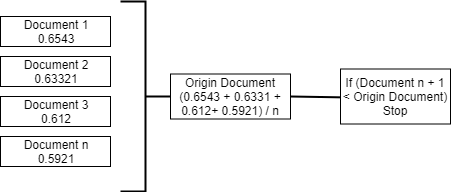
\includegraphics[height=4cm]{figures/originMethod.png}
\caption{Calculating Origin Average}
\end{figure}

The \% difference between document $n+1$ and the pseudo document would still be used to derive the stopping point.

This approach has the advantage of taking into consideration variability in the quality of the rankings. It also has the advantage of being entirely unsupervised and does not require us to sample the initial document collection. 

A further development of this method is to create an pseudo document using the document abstract text:

\begin{figure}[H]
\center
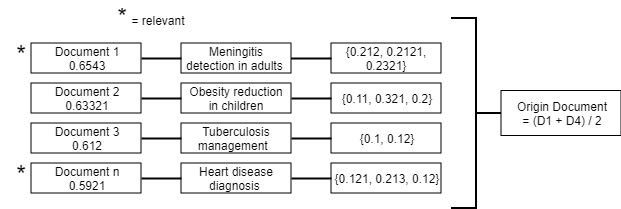
\includegraphics[height=4cm]{figures/origin2.png}
\caption{Generating Origin vector using document abstract}
\end{figure}


We have further developed the method in that we are using the top $n$ documents to calculate an average document vector by using the content of the document. We can then use vector similarity comparisons such as euclidean distance and cosine similarity to compare the origin document vector to further documents down the rankings.

This method can be tweaked and optimized by standard by applying standard text processing/NLP techniques:

\begin{itemize}
  \item Using Word2Vec to represent abstract features
  \item Language modelling abstract features, trying out different NGram sizes
  \item Pre-processing of a abstracts
  
\end{itemize}

Finally we can use the work in \ref{automatic_f_t_r} as part of this method by extracting further useful information from the full texts. This information could be used to expand the content of the abstract as-well act as a separate source for further information for finding a stopping point.


\begin{figure}[H]
\center
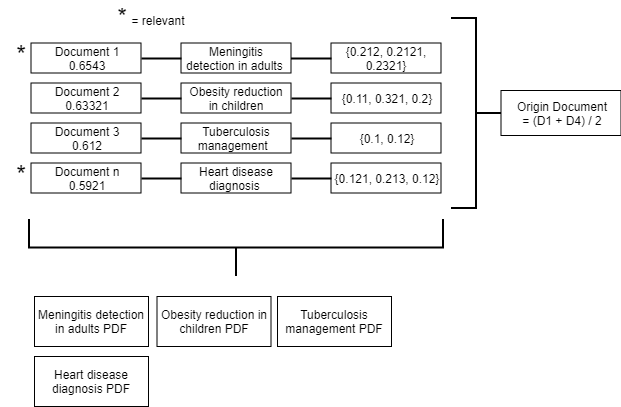
\includegraphics[height=7cm]{figures/origin3.png}
\caption{Generating Origin vector using document abstract and text}
\end{figure}


Another method to stopping that could be applied is implementing a classifier. We would still look to use the abstracts as training data for relevant and non-relevant documents. This method would assume we take a sample set of documents as our training data. This training data would then be used to build a classifier to determine if the rest of the documents are relevant or non relevant. We can infer the expected number of relevant documents from the sample and make the assumptions about how many we would need to find to attain a reliability score of 95\%.



\section{Gnatt Chart} \label{gnatt}


\begin{figure}[H]
\center
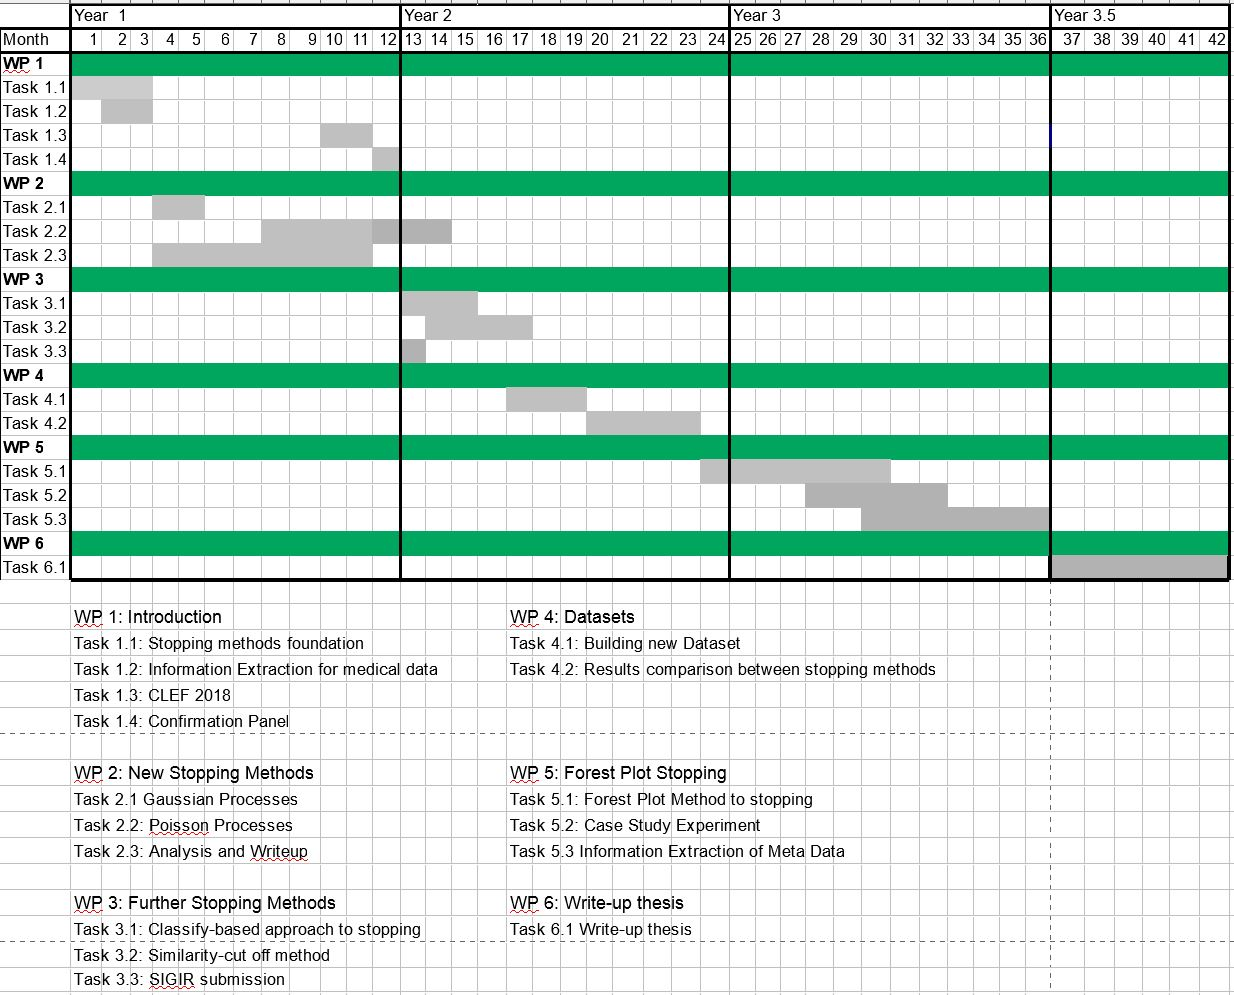
\includegraphics[height=16cm]{figures/gnatt_chart2.jpg}
\caption{Gnatt Chart}
\end{figure}

Initial work focused on background reading around stopping points as well as exploring other ideas as for applying text processing within systematic reviews.

Was able to re-implement some existing stopping methods and apply them to our own datasets.

Explored some new potential areas for stopping methods and developed some unique approaches.

Submitted a paper to CLEF 2018 and gave a talk at the conference on our methods.

Future work will expand on the similarity-cut off method to stopping \ref{fw} by using more information from the abstracts.



 \chapter{Doctorial Development Programme} \label{lit}


\begin{itemize}
  \item Attended Healtex - UK HEALTHCARE TEXT ANALYTICS CONFERENCE
  \item Lab demonstrator for module COM4519 Cloud Computing
  \item Undertook module HAR6169 Study Design and Systematic Review Methods
  \item Marked assignments for COM3110 Text Processing
  \item Enrolled on FCE6100 Professional Behaviour and Ethical Conduct
  \item Completed TRAINING NEEDS ANALYSIS (TNA) form.
  \item Used Learning Management System (LMS) too attend 6 teacher training courses.
  \item Gave introduction talk to NLP group.
  \item Contributed to 2018 CLEF lab.
  
  
\end{itemize}

 
% \chapter{Conclusions}

We first introduced the \#happysheffield web app and discussed how it is currently implemented.

We evaluated the performance of \#happysheffield using evaluation semantics. We can use this data as a base line for when we attempt to improve the performance of the web app using different affect analysis techniques.

We have revised the relevant literature that surrounds affect analysis. We have looked at different techniques we can apply, including their pros and cons. We decided which of these techniques would be suitable to apply to \#happysheffield. It was decided that we would favour supervised machine learning techniques, due to the large availability of datasets and scalability 

We looked at other potential improvements to \#happysheffield and decided to implement some extra features such as being able to compare emotion across places and displaying tweets as they arrive live from Twitter.

Finally we formally planned the project using a gnatt chart and risk assessment; identifying potential hazards and what action to take if they occur.

Overall the main objective of this project is to evaluate \#happysheffield, with a strong focus on applying modern affect analysis techniques in hope of improving the performance.




%\chapter{Results} \label{results}

This section will discuss the results of our implementations. The aim here is to improve the performance of \#happysheffield gradually. We will use the same evaluation metrics as described in the analysis of existing system

\section{Cycle One} \label{cycle_1}

For the first cycle, we created a simple Naive Bayes classifier to categorise each tweet by emotion. We used a unigram language model and words as features. We used a tokenizer designed for usage with twitter data \cite{OConnor2010}. No external libraries were used, we simply used the data types and storage classes provided by the Python programming language. No additional pre-processing or smoothing methods were applied.

We can evaluate the results by training on 75\% of the data set and using the remaining 25\% to test our system. In future, we will use cross-validation.

Using this technique we were able to achieve an overall system accuracy of \textbf{0.536}.

We can look further into the system performance by looking at the precision, recall and f-measure for each emotion.


\begin{table}[H]
\center
 \begin{tabular}{|c|c|c|c|c|c|c|} 
 \hline
 \ Evaluation & \textbf{anger} & \textbf{joy} & \textbf{fear} & \textbf{disgust} & \textbf{sadness} & \textbf{surprise} \\ [0.5ex] 
 \hline
 \ \textbf{Base Naive Bayes Classifier} & & & & & &  \\ [0.5ex] 
 \hline
 Precision & 0.468 & 0.497 & 0.803 & 1.0 & 0.552 & 0.628 \\ 
 \hline
 Recall & 0.102 & 0.928 & 0.434 & 0.0117 & 0.362 & 0.267 \\
 \hline
 F-Measure & 0.167 & 0.647 & 0.564 & 0.023 & 0.437 & 0.375 \\
 \hline
\end{tabular}
\caption{Scores for basic classifier}
\end{table}


\iffalse
\begin{figure}[H]
\center
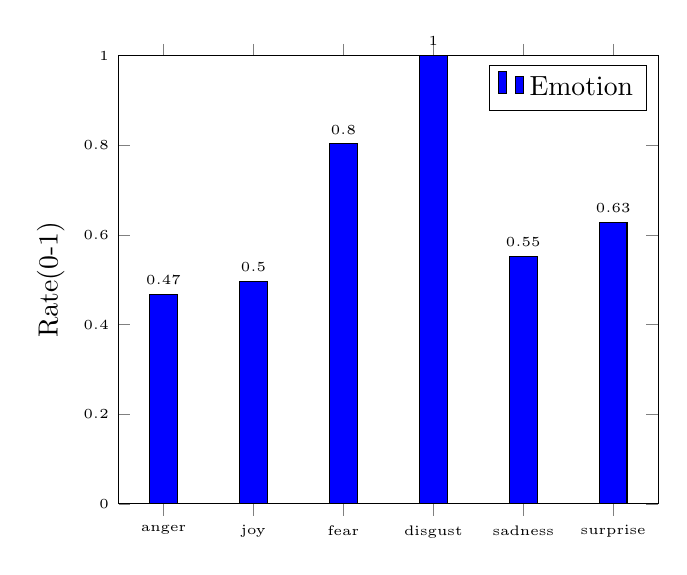
\begin{tikzpicture}
\begin{axis}[
    ymin = 0,
    ymax = 1,
    symbolic x coords={anger,joy,fear,disgust,sadness,surprise},
    xtick=data,
    ybar = 2.2,
    ylabel=Rate(0-1),
    nodes near coords,
    scaled x ticks = false,
    tick label style={font=\tiny} ,
    every node near coord/.style={/pgf/number format/fixed, font=\tiny},
]
\addplot [ybar, fill=blue]
    coordinates {
        (anger,0.468) (joy,0.497)
         (fear,0.803) (disgust,1.0) (sadness, 0.552) (surprise, 0.628)
         
         };
\legend{Emotion}
\title{Precision Rates}
\end{axis}
\end{tikzpicture}
\caption{The precision rates for each emotion class[Naive Bayes][C1]}
\end{figure}

\begin{figure}[H]
\center
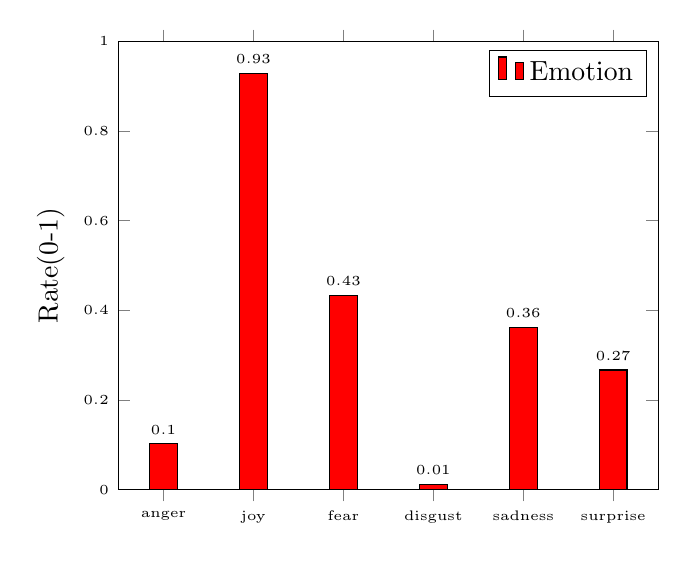
\begin{tikzpicture}
\begin{axis}[
    ymin = 0,
    ymax = 1,
    symbolic x coords={anger,joy,fear,disgust,sadness,surprise},
    xtick=data,
    ybar = 2.2,
    ylabel=Rate(0-1),
    nodes near coords,
    scaled x ticks = false,
    tick label style={font=\tiny} ,
    every node near coord/.style={/pgf/number format/fixed, font=\tiny},
]
\addplot [ybar, fill=red]
    coordinates {
        (anger,0.102) (joy,0.928)
         (fear,0.434) (disgust,0.0117) (sadness, 0.362) (surprise, 0.267)
         
         };
\legend{Emotion}
\title{Recall Rates}
\end{axis}
\end{tikzpicture}
\caption{The recall rates for each emotion class[Naive Bayes][C1]}
\end{figure}



\begin{figure}[H]
\center
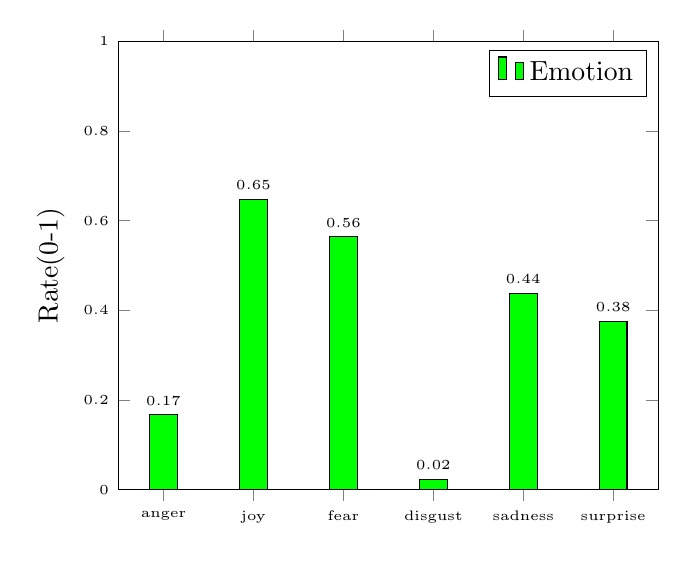
\begin{tikzpicture}
\begin{axis}[
    ymin = 0,
    ymax = 1,
    symbolic x coords={anger,joy,fear,disgust,sadness,surprise},
    xtick=data,
    ybar = 2.2,
    ylabel=Rate(0-1),
    nodes near coords,
    scaled x ticks = false,
    tick label style={font=\tiny} ,
    every node near coord/.style={/pgf/number format/fixed, font=\tiny},
]
\addplot [ybar, fill=green]
    coordinates {
        (anger,0.167) (joy,0.647)
         (fear,0.564) (disgust,0.023) (sadness, 0.437) (surprise, 0.375)
         
         };
\legend{Emotion}
\title{F-Measure Rates}
\end{axis}
\end{tikzpicture}
\caption{The F-Measure rates for each emotion class[Naive Bayes][C1]}
\end{figure}

\fi

We can see that our results are highly varied between different emotions. Disgust achieved a 1.0 rate for precision, but this was because our classifier only gave 1 of the 85 disgust tweets this emotion and resulted in a very small recall.

Joy is the most commonly assigned emotion; we managed to assign 738 of the 795 joy tweets. But our system over-classifies this emotion too, as it gave 1484 tweets a joy assignment, despite there only being 795 joy tweets in our test set. 

Overall our machine-learning based implementation performs better than the lexicon based approach, but the quality of results for each emotion type is more varied.


\subsection{Cycle One Conclusion}

We were able to improve the overall system accuracy from \textbf{0.313} to \textbf{0.536}. This is a good start, but we can see our system is over-classifying tweets of the joy emotion and severely under-classifying tweets of the disgust emotion. We are also not doing any pre-processing or handling more sophisticated language, such as negation. This will be the focus on subsequent sections. 

\section{Cycle Two} \label{cy2}

The decision was taken to use a more optimized toolkit for implementing our classifier. scikit-learn \cite{scikit} provides an optimized a series of optimized methods for implementing machine learning algorithms.

Our next implementation uses Multinomial Naive Bayes provided by scikit-learn along with a stop-list and +1 smoothing. We used unigram features along with the same tokenizer described in the cycle one. We are also representing words as simple count vectors, e.g.,

\begin{center}
\textit {\@william "I am happy happy happy today"}
\end{center}

\begin{equation} \label{count_vector}
S = {1,1,3,1}
\end{equation}

We applied 10-folds of cross validation to evaluate the performance.

Using this technique we were able to achieve an overall average system accuracy of \textbf{0.558}. We calculated this as the sum of the accuracy for each fold, normalized by the number of folds and can be described formally as follows:

\begin{equation}
A = \frac{\sum_{f_i}^{F}}{F}
\end{equation}

Where $F$ is the number of folds and $A$ is the average accuracy.

We can calculate the average precision, recall, and f-measure by applying the same formula. We can then compare our new system to our legacy Naive Bayes implementation.



\begin{table}[H]
\center
 \begin{tabular}{|c|c|c|c|c|c|c|} 
 \hline
 \ Evaluation & \textbf{anger} & \textbf{joy} & \textbf{fear} & \textbf{disgust} & \textbf{sadness} & \textbf{surprise} \\ [0.5ex] 
 \hline
 \ \textbf{Base Naive Bayes Classifier} & & & & & &  \\ [0.5ex] 
 \hline
 Precision & 0.468 & 0.497 & 0.803 & 1.0 & 0.552 & 0.628 \\ 
 \hline
 Recall & 0.102 & 0.928 & 0.434 & 0.0117 & 0.362 & 0.267 \\
 \hline
 F-Measure & 0.167 & 0.647 & 0.564 & 0.023 & 0.437 & 0.375 \\
 \hline
 \ \textbf{NB,Scikit,Stoplist,Smoothing} & & & & & &  \\ [0.5ex] 
 \hline
  Precision & 0.654 & 0.534 & 0.718 & 0.886 & 0.487 & 0.675 \\ 
 \hline
 Recall & 0.172 & 0.91 & 0.487 & 0.047 & 0.362 & 0.311 \\
 \hline
 F-Measure & 0.273 & 0.647 & 0.564 & 0.087 & 0.415 & 0.425 \\
 \hline
\end{tabular}
\caption{Scores for basic classifier}
\end{table}

\iffalse
\begin{figure}[H]
\center
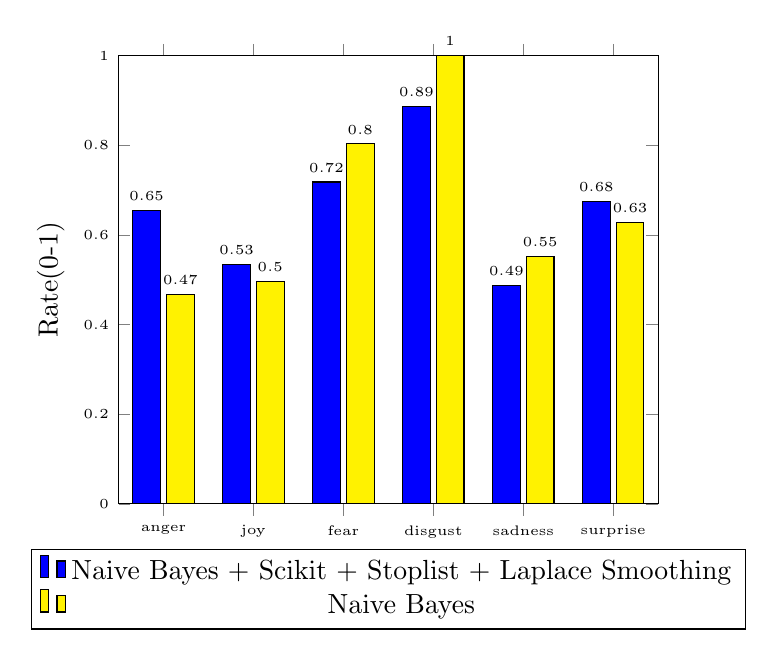
\begin{tikzpicture}
\begin{axis}[
    ymin = 0,
    ymax = 1,
    legend style={at={(0.5,-0.1)},
    anchor=north,legend columns=1},
    symbolic x coords={anger,joy,fear,disgust,sadness,surprise},
    xtick=data,
    ybar = 2.2,
    ylabel=Rate(0-1),
    nodes near coords,
    scaled x ticks = false,
    tick label style={font=\tiny} ,
    every node near coord/.append style={/pgf/number format/fixed, font=\fontsize{1}{1}\selectfont},
]
\addplot [ybar, fill=blue]
    coordinates {
        (anger,0.654) (joy,0.534)
         (fear,0.718) (disgust,0.886) (sadness, 0.487) (surprise, 0.675)
         
         };
         
\addplot [ybar, fill=yellow]
    coordinates {
        (anger,0.468) (joy,0.497)
         (fear,0.803) (disgust,1.0) (sadness, 0.552) (surprise, 0.628)
         
         };
\addlegendentry{Naive Bayes + Scikit + Stoplist + Laplace Smoothing}
\addlegendentry{Naive Bayes}
\title{Precision Rates}
\end{axis}
\end{tikzpicture}
\caption{Comparison of precision rates for each emotion class[Naive Bayes][C2] and scikit learn}
\end{figure}


\begin{figure}[H]
\center
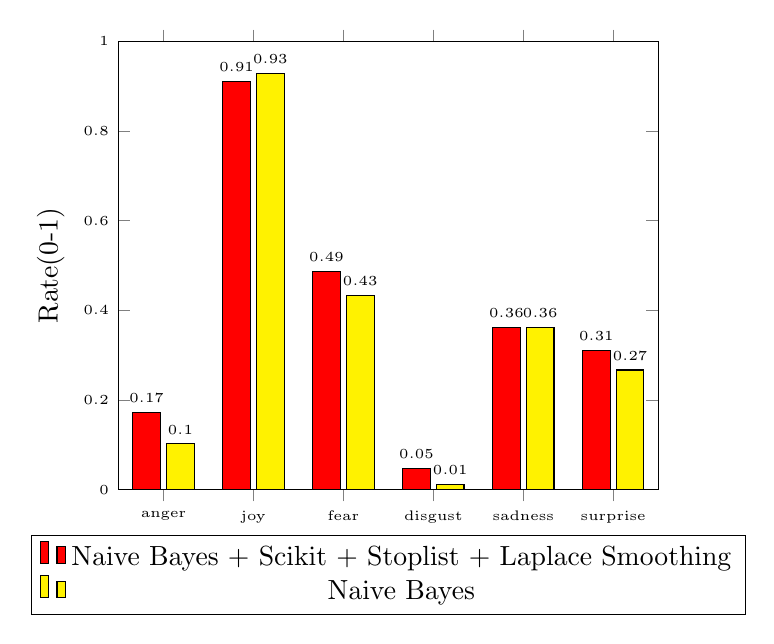
\begin{tikzpicture}
\begin{axis}[
        ymin = 0,
    ymax = 1,
    legend style={at={(0.5,-0.1)},
    anchor=north,legend columns=1},
    symbolic x coords={anger,joy,fear,disgust,sadness,surprise},
    xtick=data,
    ybar = 2.2,
    ylabel=Rate(0-1),
    nodes near coords,
    scaled x ticks = false,
    tick label style={font=\tiny} ,
    every node near coord/.append style={/pgf/number format/fixed, font=\fontsize{1}{1}\selectfont},
]
\addplot [ybar, fill=red]
    coordinates {
        (anger,0.172) (joy,0.91)
         (fear,0.487) (disgust,0.047) (sadness,0.362) (surprise, 0.311)
         
         };
\addplot [ybar, fill=yellow]
    coordinates {
        (anger,0.102) (joy,0.928)
         (fear,0.434) (disgust,0.0117) (sadness, 0.362) (surprise, 0.267)
         
         };
\addlegendentry{Naive Bayes + Scikit + Stoplist + Laplace Smoothing}
\addlegendentry{Naive Bayes}
\title{Recall Rates}
\end{axis}
\end{tikzpicture}
\caption{Comparison of recall rates for each emotion class[Naive Bayes][C2] and scikit learn}
\end{figure}

\begin{figure}[H]
\center
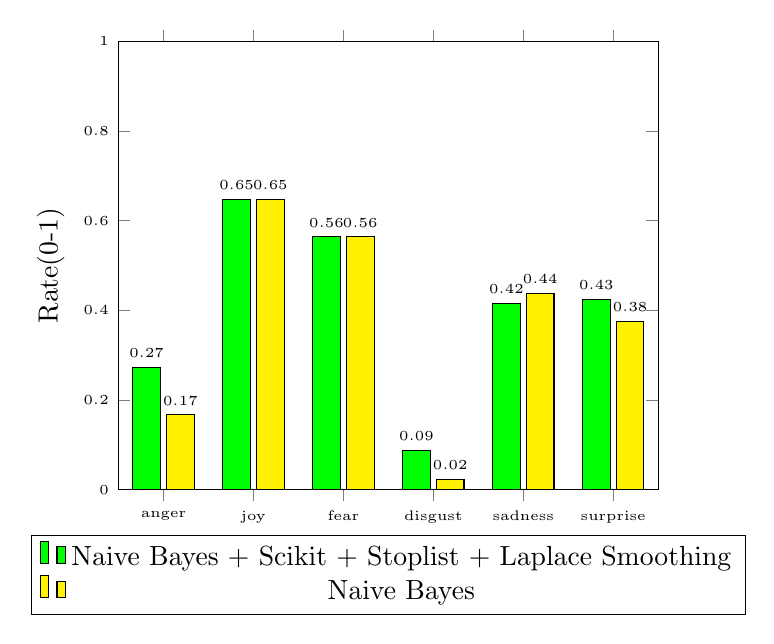
\begin{tikzpicture}
\begin{axis}[
        ymin = 0,
    ymax = 1,
    legend style={at={(0.5,-0.1)},
    anchor=north,legend columns=1},
    symbolic x coords={anger,joy,fear,disgust,sadness,surprise},
    xtick=data,
    ybar = 2.2,
    ylabel=Rate(0-1),
    nodes near coords,
    scaled x ticks = false,
    tick label style={font=\tiny} ,
    every node near coord/.append style={/pgf/number format/fixed, font=\fontsize{1}{1}\selectfont},
]
\addplot [ybar, fill=green]
    coordinates {
        (anger,0.273) (joy,0.647)
         (fear,0.564) (disgust,0.087) (sadness, 0.415) (surprise, 0.425)
         
         };
         
\addplot [ybar, fill=yellow]
    coordinates {
        (anger,0.167) (joy,0.647)
         (fear,0.564) (disgust,0.023) (sadness, 0.437) (surprise, 0.375)
         
         };
\addlegendentry{Naive Bayes + Scikit + Stoplist + Laplace Smoothing}
\addlegendentry{Naive Bayes}
\title{F-Measure Rates}
\end{axis}
\end{tikzpicture}
\caption{Comparison of F-Measure rates for each emotion class[Naive Bayes][C2] and scikit learn}
\end{figure}

\fi

We can see that we have improved the overall performance of the majority of emotions. Sadness slightly suffered, but all the other emotions saw increased performance.

The precision rate has dropped for fear, disgust, sadness, and surprise this is not necessarily a bad thing as it means our system is now putting in more effort in classifying for these emotions.

Anger, surprise, disgust, and fear have all had good recall rate increases, but joy has lost some recall rate.(this was to be expected as the value was too high sustain while improving the other emotions)

We still have the same problem in that joy is receiving over-classification and disgust is not receiving under-classification.

\subsection{Vector Representation} \label{vec_rep}

We discussed earlier how we are representing tweets as simple count vectors \ref{count_vector}. There are alternative approaches to representing tweets. 

One approach we can take is to use the tf-idf weighting scheme, commonly used in information retrieval. The idea behind tf-idf is that we combine both the term frequency and inverse document frequency to get a value. tf is simply the number of times the term appears in the tweet. idf is a value for scoring the importance of a term in a tweet; more common words receive a lower value, more information-bearing terms receive a higher value.

sci-kit learn provides an easy way to represent our training data in tf-idf format. We replaced our count vectorizer with the tf-idf equivalent and took the average accuracy. The average accuracy dropped to \textbf{0.483}. Further investigation discovered that this weighting scheme in not suitable for our task. This is because terms like 'happy' and 'sad' are given low values by the idf weighting, despite being of importance to the classification of the tweet. It was also put the recall down to $<$ 0.24 for all emotions (apart from joyful).

\subsection{Naive Bayes Variations}

So far we have been using a multinomial naive bayes classifier. This works well in our situation as we are using word counts to classify text.

The Bernoulli variant assumes binary vectors; rather than counts. This means if a word is contained within a tweet it gets a 1 value; else it gets a 0 value. This variant makes little impact on the system as tweets are small messages and are unlikely to the same content-bearing word more than once.

Due to the nature of social media data, the vocabulary range is large for our twitter dataset. Research suggests that the multinomial variant of naive bayes performances better than the Bernoulli varient, when the vocabulary range is large \cite{mccallum1998comparison}. For this reason, the decision was taken to stick to the multinomial variant.

\subsection{Over-classification Problem}

One problem with our training data is that it is not evenly distributed, we have much more joyful tweets than any others. This is resulting in an over-classification towards the joyful emotion. The Naive Bayes classifier has two parts; the likelihood and the prior. The prior will give a higher weighting to more common classes, emitting the prior will mean all classes of equal initial likelihood.

With this in mind, we can run another evaluation without the prior. This increase our average accuracy from \textbf{0.558} to \textbf{0.575}. 

We can also see how they affect the F-Score

\begin{figure}[H]
\center
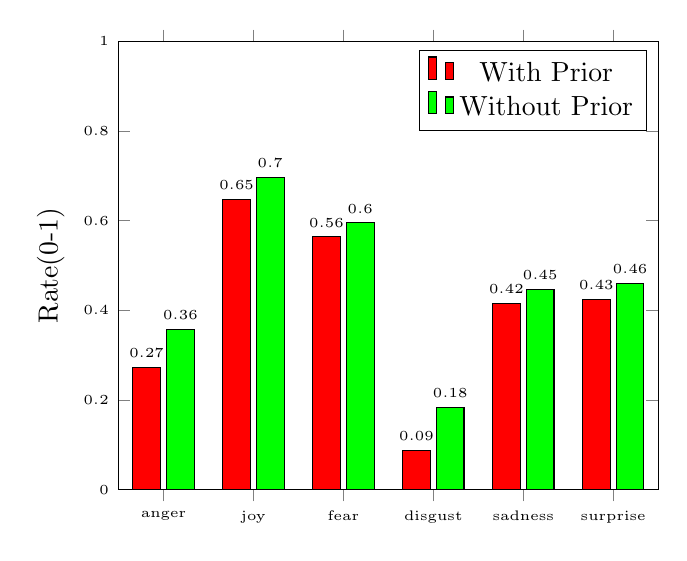
\begin{tikzpicture}
\begin{axis}[
    ymin = 0,
    ymax = 1,
    symbolic x coords={anger,joy,fear,disgust,sadness,surprise},
    xtick=data,
    ylabel=Rate(0-1),
    compat=newest, %Better label placement,
    ybar = 2.2,
    nodes near coords,
    scaled x ticks = false,
    tick label style={font=\tiny} ,
    every node near coord/.append style={/pgf/number format/fixed, font=\fontsize{1}{1}\selectfont},
]


\addplot [ybar, fill=red]
    coordinates {
        (anger,0.273) (joy,0.647)
         (fear,0.564) (disgust,0.087) (sadness, 0.415) (surprise, 0.425)
         
         };
         
\addplot [ybar, fill=green]
    coordinates {
        (anger,0.358) (joy,0.697)
         (fear,0.595) (disgust,0.183) (sadness, 0.447) (surprise, 0.460)
         };
         
                     
\addlegendentry{With Prior}
\addlegendentry{Without Prior}
\title{F-Measure Rates}
\end{axis}
\end{tikzpicture}
\caption{Comparison of F-Measure rates for each emotion class[Naive Bayes][C2] with and without prior}
\end{figure}

We can see our system improves for each emotion when emitting the prior. The disgust emotion doubles in performance; meaning our system is now doing a better job at assigning this emotion.

Our average recall rate for the joy emotion has also dropped down to 0.85. Which again is not a bad thing as it means our system is being less bias towards this emotion.

\subsection{Cycle Two Conclusion}

We were able to improve the performance of the system by using scikit learn along with a stoplist and basic Laplace smoothing. We then began to look at how we can solve the problem of bias towards certain classes. We established that we could emit the prior from our naive bayes system to get a better overall system performance. Next, we looked at how we can represent tweets as both count vectors and tf-idf values, but established count vectors work best.

The next cycle will look at more techniques we can apply to improve the performance.

\section{Cycle Three} \label{cy3}

When pre-processing our tweets, there are numerous things we can do to improve the performance. Some things we can include are:
\begin{itemize}
    \item Resolve excessive characters e.g 'hiiiiiii' = 'hi'
    \item Stemming terms
    \item Spelling correction
    \item Adjusting ngram size
    \item Applying a minimum document frequency (i.e a word token must appear five times across all of our training data)
\end{itemize}
\bigskip

We applied the following pre-processing techniques and then took the results:

\subsection{Elongation} \label{Elong}

Without pre-processing, tweets contain a vast vocabulary. We end up with many unique terms. It's very common to see tweets that contain excessive characters that we could resolve to just one. Consider this tweet:

\begin{center}
\textit {141003101900509186:    went out shopping for gina's birthday things loool     :: surprise}
\end{center}

We can resolve the excessive `o' in `loool` using a simple regular expression. 

\subsection{Stemming} \label{stemming_pre}

Phrases and terms can often take different forms but can be used to denote the same sentiment. We want to be able to resolve these terms to a standard form. There are many good stemmers and lemmatizers we can use for resolving the tokens of a tweet.  After comparing 3 stemmers and a lemmatizer, we found that the nltk wordnet porter stemmer yielded the best results for twitter data. \ref{comp_stem}

\subsection{ngram size} \label{ngram_size_proc}

Previously we tokenized our tweet content on single tokens (unigrams). We can adjust our processing to tokenize on larger ngrams such as bigrams and trigrams. This increases the amount tokens in our training data exponentially to our ngram size, but has the potential to handle common phrases better. Consider the following phrase:

\begin{center}
\textit {I am not happy today}
\end{center}

Our unigram implementation would leave us five tokens, one for each word.

A bigram would leave us with 5-7 tokens (depending if we wanted to handle sentence start and sentence end tokens). Importantly the phrase `not happy' would be processed as a single token.

We established that the best range of ngrams to use was an unigram-bigram combination; meaning we use both unigrams and bigrams when processing a tweet \ref{ngram}.

\subsection{Minimum df} \label{min_df_pro}

Despite us resolving excessive characters, there are still many unique terms in twitter data. These unique terms that occur only once or twice across the entire document collection often do not provide any useful knowledge of sentiment towards new information. For this reason, we can filter out tokens that occur less than a certain threshold. We found that applying a minimum document frequency of 2 yielded the best result when using multinomial naive bayes, but when using Stochastic gradient descent a minimum frequency of 1 (all terms) produced the best results. \ref{df}

\subsection{Classifier} \label{classifier_pro}

So far all of our results have been based on the fact we are using a naive bayes classifier. We can also apply other other machine learning algorithms. We will present these results in the form of confusion matrices for readability. All previously mentioned pre processing techniques \ref{min_df_pro} \ref{ngram_size_proc} \ref{stemming_pre} \ref{Elong} should be assumed to be in use, unless otherwise stated

\subsubsection{Random Forest}

\begin{figure}[H]
\center
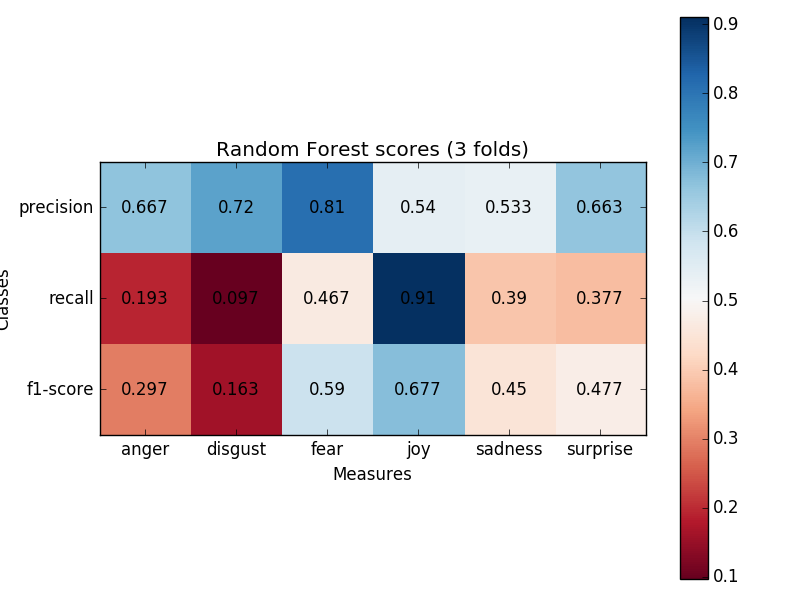
\includegraphics[width=10cm]{images/random_forest_matrix.png}
\caption{Confusion Matrix for Random Forest Classifier}
\end{figure}

The random forest classifier achieves good precision in it's predictions. But as a consequence, the recall is much lower than other classifiers. The overage system accuracy over 3 folded evaluation using random forest was \textbf{0.5759}.

\subsubsection{Decision Tree}

\begin{figure}[H]
\center
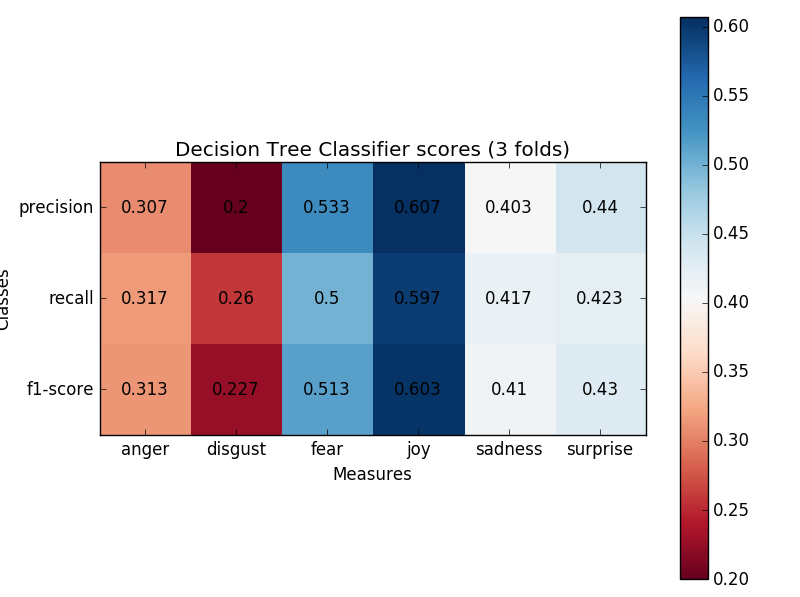
\includegraphics[width=10cm]{images/d_tree_matrix.png}
\caption{Confusion Matrix for Decision Tree Classifier}
\end{figure}

We adjusted the decision tree classifier to apply an even balance class weight. This is because the classifier favours more common emotions and results in 0 recall scores for surprise, disgust and anger. The overage system accuracy over 3 folded evaluation using decision trees was \textbf{0.4868}.

\subsubsection{Stochastic Gradient Descent}

\begin{figure}[H]
\center
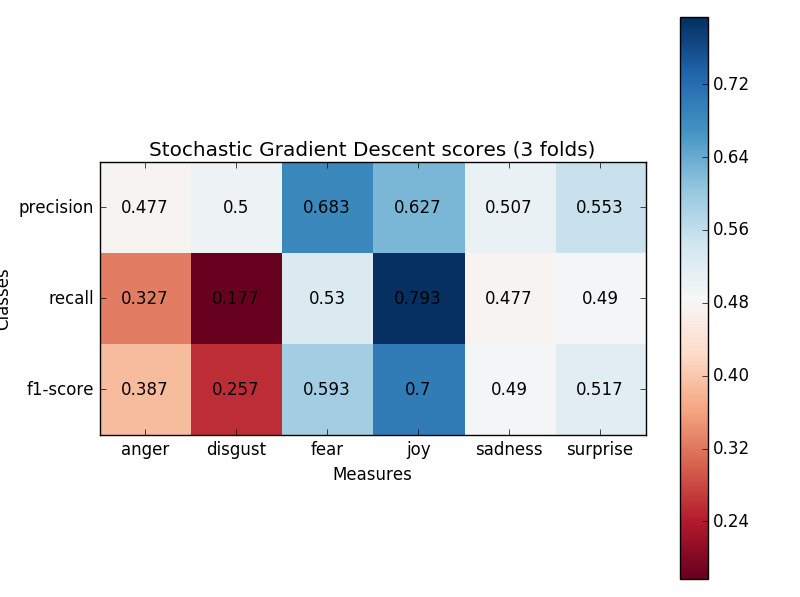
\includegraphics[width=10cm]{images/SGD_matrix.png}
\caption{Confusion Matrix for SGD Classifier}
\end{figure}

We adjusted the minimum document frequency to 1 (all terms), as it was found to improve the performance \ref{df}. Overall system accuracy \textbf{0.5891}.

\subsubsection{Multinomial Naive Bayes}

\begin{figure}[H]
\center
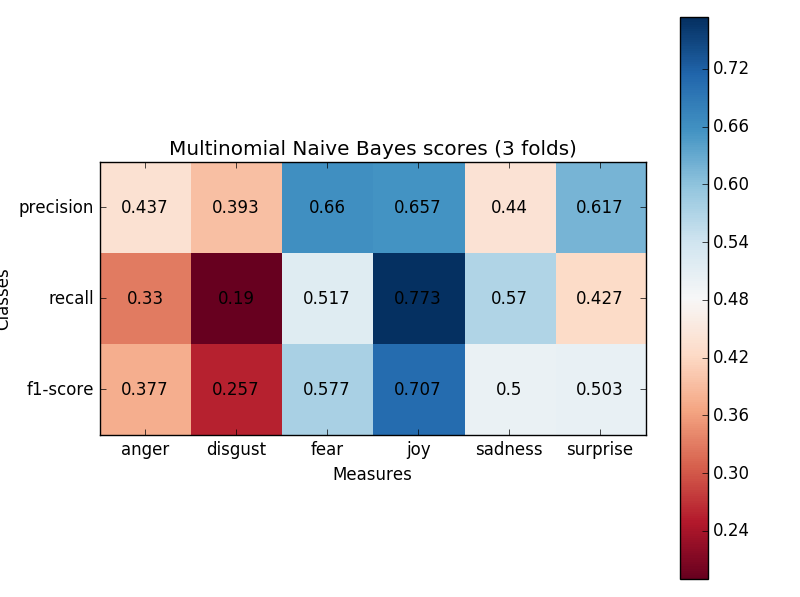
\includegraphics[width=10cm]{images/MNB_matrix.png}
\caption{Confusion Matrix for Multinomial Naive Bayes Classifier}
\end{figure}

We can see that overall we have improved the performance significantly when applying additional pre-processing techniques to the naive bayes classifier. Disgust-which was our lowest performing emotion- has gone from a 0.09 F-Measure to 0.257. This has come at some cost, however, as we can see the precision has gone down for four of the six emotions. Over 3 folds the accuracy is \textbf{0.5837}.


\iffalse
\begin{table}[H]
\center
 \begin{tabular}{|c|c|c|c|c|c|c|} 
 \hline
 \ Evaluation & \textbf{anger} & \textbf{joy} & \textbf{fear} & \textbf{disgust} & \textbf{sadness} & \textbf{surprise} \\ [0.5ex] 
 \hline
 \ \textbf{NB,Scikit,Stoplist,Smoothing} & & & & & &  \\ [0.5ex] 
 \hline
  Precision & 0.654 & 0.534 & 0.718 & 0.886 & 0.487 & 0.675 \\ 
 \hline
 Recall & 0.172 & 0.91 & 0.487 & 0.047 & 0.362 & 0.311 \\
 \hline
 F-Measure & 0.273 & 0.647 & 0.564 & 0.087 & 0.415 & 0.425 \\
 \hline
 \ \textbf{SGD,Scikit,Stoplist,Smoothing,} & & & & & &  \\ [0.5ex] 
  \hline
  \ \textbf{Stemming,DF Restriction} & & & & & & \\ [0.5ex] 
  \hline
  Precision & 0.509 & 0.642 & 0.666 & 0.393 & 0.532 & 0.557 \\ 
 \hline
 Recall & 0.301 & 0.804 & 0.537 & 0.197 & 0.486 & 0.512 \\
 \hline
 F-Measure & 0.376 & 0.713 & 0.594 & 0.281 & 0.415 & 0.425 \\
 \hline
 \ \textbf{NB,Scikit,Stoplist,Smoothing,} & & & & & &  \\ [0.5ex] 
  \hline
  \ \textbf{Stemming,DF Restriction} & & & & & & \\ [0.5ex] 
  \hline
 F-Measure & 0.36 & 0.718 & 0.575 & 0.205 & 0.514 & 0.524 \\
 \hline
 
\end{tabular}
\caption{Scores for basic classifier}
\end{table}
\fi

\iffalse

\begin{figure}[H]
\center
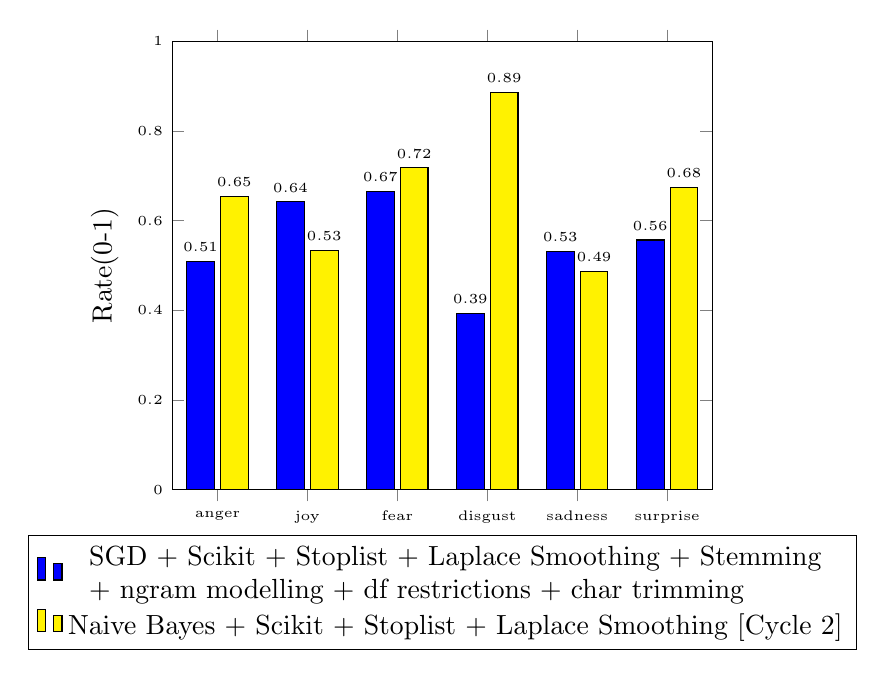
\begin{tikzpicture}
\begin{axis}[
    ymin = 0,
    ymax = 1,
    legend style={at={(0.5,-0.1)},
    anchor=north,legend columns=1},
    symbolic x coords={anger,joy,fear,disgust,sadness,surprise},
    xtick=data,
    ybar = 2.2,
    ylabel=Rate(0-1),
    nodes near coords,
    scaled x ticks = false,
    tick label style={font=\tiny} ,
    every node near coord/.append style={/pgf/number format/fixed, font=\fontsize{1}{1}\selectfont},
]

\addplot [ybar, fill=blue]
    coordinates {
        (anger,0.509) (joy,0.642)
         (fear,0.666) (disgust,0.393) (sadness, 0.532) (surprise, 0.557)
         
         };
                  
\addplot [ybar, fill=yellow]
    coordinates {
        (anger,0.654) (joy,0.534)
         (fear,0.718) (disgust,0.886) (sadness, 0.487) (surprise, 0.675)
         
         };
         
\addlegendentry[align=left]{SGD + Scikit + Stoplist + Laplace Smoothing + Stemming \\ + ngram modelling + df restrictions + char trimming}
\addlegendentry[align=left]{Naive Bayes + Scikit + Stoplist + Laplace Smoothing [Cycle 2]}
\title{Precision Rates}
\end{axis}
\end{tikzpicture}
\caption{Comparison of precision rates for each emotion class using SGD along with stemming, ngram modelling, df restrictions and excessive character trimming}
\end{figure}




\begin{figure}[H]
\center
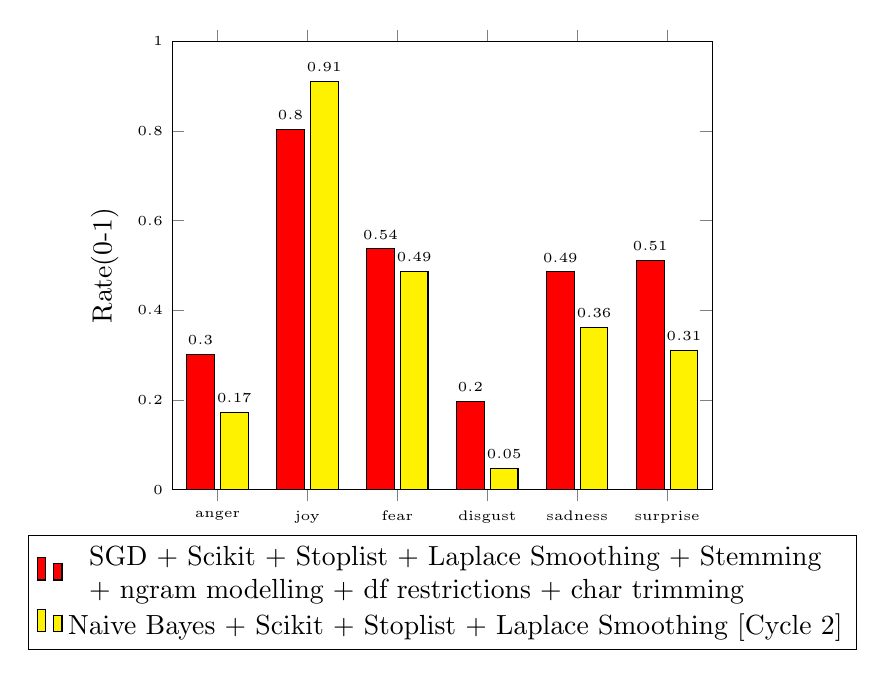
\begin{tikzpicture}
\begin{axis}[
        ymin = 0,
    ymax = 1,
    legend style={at={(0.5,-0.1)},
    anchor=north,legend columns=1},
    symbolic x coords={anger,joy,fear,disgust,sadness,surprise},
    xtick=data,
    ybar = 2.2,
    ylabel=Rate(0-1),
    nodes near coords,
    scaled x ticks = false,
    tick label style={font=\tiny} ,
    every node near coord/.append style={/pgf/number format/fixed, font=\fontsize{1}{1}\selectfont},
]


\addplot [ybar, fill=red]
    coordinates {
        (anger,0.301) (joy,0.804)
         (fear,0.537) (disgust,0.197) (sadness,0.486) (surprise, 0.512)
         
         };
         
\addplot [ybar, fill=yellow]
    coordinates {
        (anger,0.172) (joy,0.91)
         (fear,0.487) (disgust,0.047) (sadness,0.362) (surprise, 0.311)
         
         };
\addlegendentry[align=left]{SGD + Scikit + Stoplist + Laplace Smoothing + Stemming \\ + ngram modelling + df restrictions + char trimming}
\addlegendentry[align=left]{Naive Bayes + Scikit + Stoplist + Laplace Smoothing [Cycle 2]}
\title{Recall Rates}
\end{axis}
\end{tikzpicture}
\caption{Comparison of recall rates for each emotion class using SGD along with stemming, ngram modelling, df restrictions and excessive character trimming}
\end{figure}


\begin{figure}[H]
\center
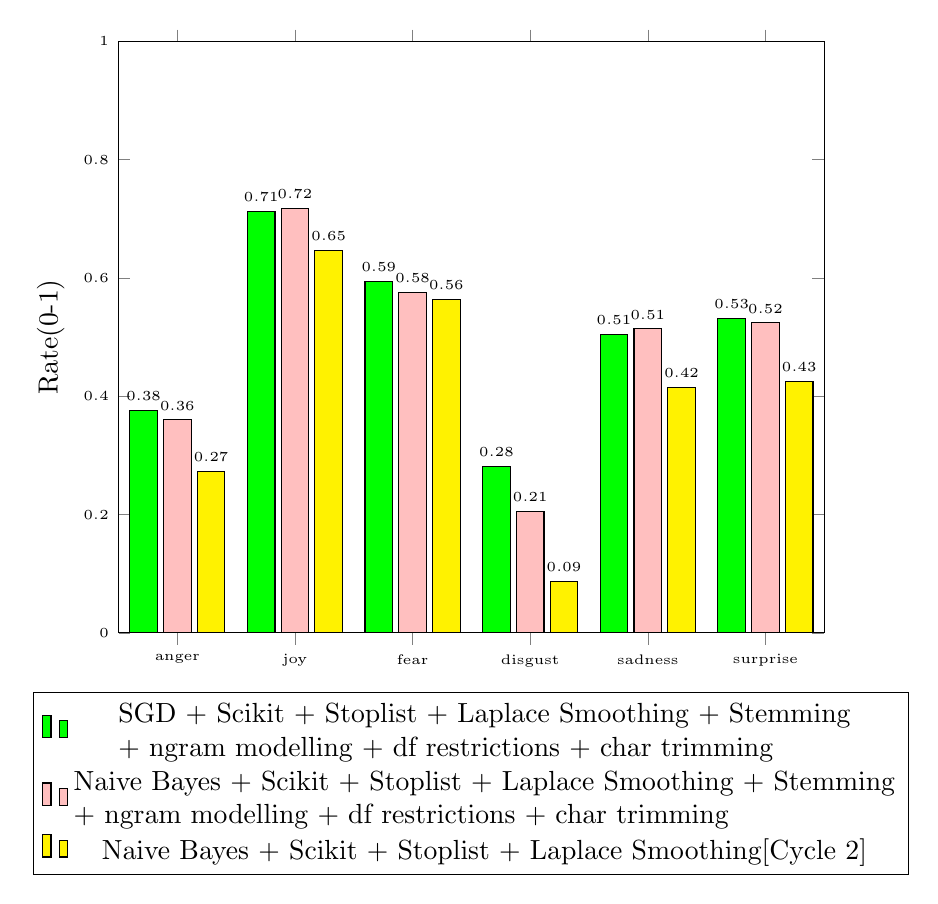
\begin{tikzpicture}
\begin{axis}[
        ymin = 0,
    ymax = 1,
    width = 300,
    legend style={at={(0.5,-0.1)},
    anchor=north,legend columns=1},
    symbolic x coords={anger,joy,fear,disgust,sadness,surprise},
    xtick=data,
    ybar = 2.2,
    ylabel=Rate(0-1),
    nodes near coords,
    scaled x ticks = false,
    tick label style={font=\tiny} ,
    every node near coord/.append style={/pgf/number format/fixed, font=\fontsize{1}{1}\selectfont},
]

\addplot [ybar, fill=green]
    coordinates {
        (anger,0.376) (joy,0.713)
         (fear,0.594) (disgust,0.281) (sadness, 0.505) (surprise, 0.532)
         
         };
         
\addplot [ybar, fill=pink]
    coordinates {
        (anger,0.36) (joy,0.718)
         (fear,0.575) (disgust,0.205) (sadness, 0.514) (surprise, 0.524)
         
         };

\addplot [ybar, fill=yellow]
    coordinates {
        (anger,0.273) (joy,0.647)
         (fear,0.564) (disgust,0.087) (sadness, 0.415) (surprise, 0.425)
         
         };
         

\addlegendentry[align=left]{SGD + Scikit + Stoplist + Laplace Smoothing + Stemming \\ + ngram modelling + df restrictions + char trimming}

\addlegendentry[align=left]{Naive Bayes + Scikit + Stoplist + Laplace Smoothing + Stemming \\ + ngram modelling + df restrictions + char trimming}

\addlegendentry[align=left]{Naive Bayes + Scikit + Stoplist + Laplace Smoothing[Cycle 2]}
\title{F-Measure Rates}
\end{axis}
\end{tikzpicture}
\caption{Comparison of F-measure rates for each emotion class using SGD along with stemming, ngram modelling, df restrictions and excessive character trimming}
\end{figure}
\fi


\subsubsection{Classifier Conclusion}

The gradient decent classifier performs the best overall, but the results are negligible. We have decided to stay with our naive bayes classifier as the model made it easier for us to append additional factors as we will see later. \ref{log_model}

\section{Cycle 4}

We can now look at some more features to improve the overall performance of our system.

\subsection{Subjectivity}

As it stands, our system will attempt to classify every tweet that it receives. Some tweets, however, are not necessarily portraying any emotion. For this reason, we can introduce a subjectivity analyser against the tweet. The goal here is to classify the tweet as either subjective or objective. Subjective tweets continue down our processing channel and receive an emotion classification, while objective tweets are discarded.

There are many different ways we can go about subjectivity analysis. A supervised machine learning approach would require training data of subjective and objective tweets. A dataset provided here \cite{baccianella2010sentiwordnet} contains a list of tweets along with 0-1 positive-negative scores, scores with a value of 0 can be assumed to be objective.

A convenient NLP library called TextBlob \cite{textblob} provides an easy way of classifying documents as subjective or as objective. The library provides a method for generating the subjectivity; it returns a value between 0.0 and 1.0 where 0.0 is certainly objective, and 1.0 is certainly subjective.

We can evaluate the performance by running the wordnet tweet dataset through an evaluation. We can then look at what is the best cut-off point for determining if a tweet is subjective or objective.

A cut-off point is what determines when we decide if we should count the tweet as subjective. For instance, a 0.9 cut-off point would mean only tweets with a subjectivity score greater than 0.9 are considered subjective.

\begin{figure}[H]
\center
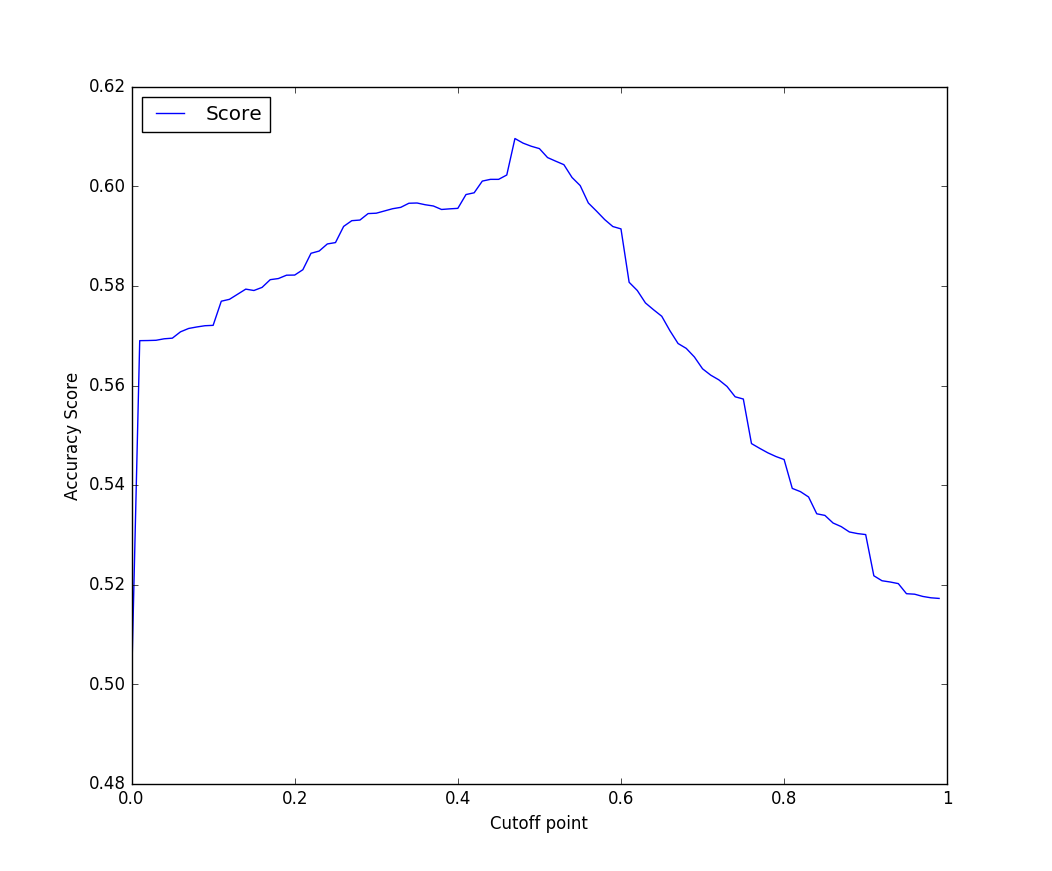
\includegraphics[width=13cm]{figures/subjectiveTest.png}
\caption{Accuracy score of TextBlob\cite{textblob} compared between cut-off points}
\end{figure}

Fig 6.8 shows how varying the cut-off point effects the accuracy of the classification for the subjectivity of tweets using TextBlob\cite{textblob}. 

Using this method we achieve a subjectivity classifier accuracy for tweets of \textbf{0.609} at \textbf{0.47} cut-off point.

It should be noted that in practice we should try to classify as many tweets as possible, as we're trying to calculate the overall emotion of Sheffield. Deliberately filtering out tweets could restrict the overall activity of the platform. For this reason, the decision has been taken to run the subjectivity classifier, but not filter out any tweets.

\section{Cycle 5} \label{c5}

A major limitation of our training data is that it is old. Twitter data has a broad domain and users can be discussing a huge range of topics. Some topics invoke different emotions at certain points in time; making it difficult to determine the emotion of a new tweet. Consider a political figure who may be very popular when elected, but peoples' emotions could change as time progresses.

There is another problem with our training data in that it does not contain emojis. Emojis can be of use when trying to learn the emotion of a tweet. A study here \cite{novak2015sentiment} looked at how accurate an emoji can be in reflecting the polarity of the tweet (negative,neutral and positive)

\begin{figure}[H]
\center
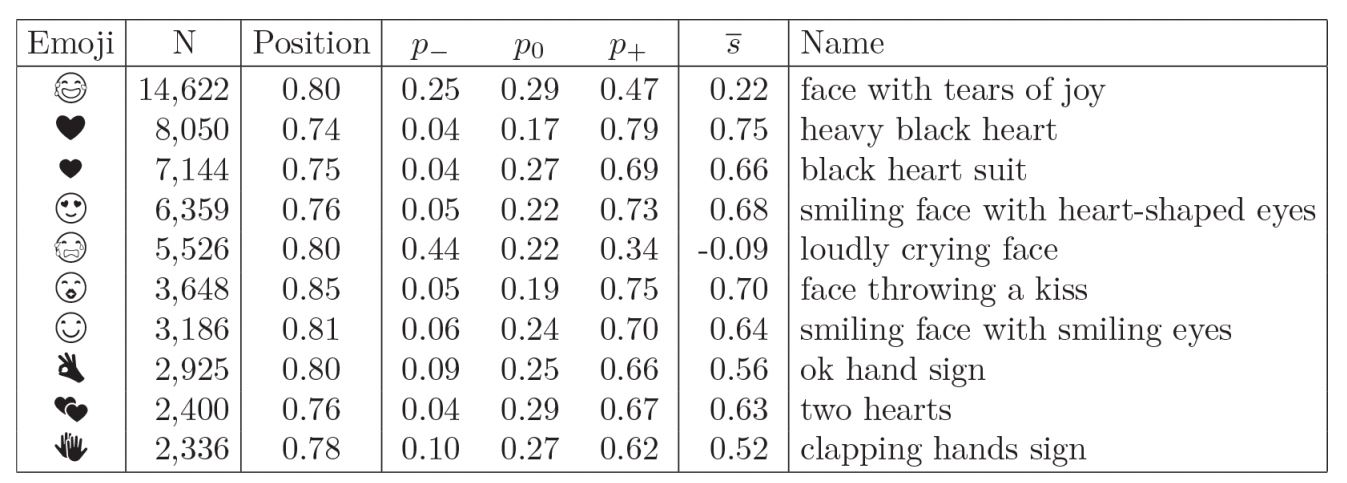
\includegraphics[width=15cm]{images/emojj_table.JPG}
\caption{Emojjs relation to tweet polarity. Table reproduced from \cite{novak2015sentiment}}
\end{figure}

$(p−, p0, p+).$ form a probability distribution for positive, neutral and negative emotions respectively. We can see that the `heavy black heart' emoji often occurs in positive tweets (0.79 rate)

With this in mind, this cycle will look at how we can obtain and use more up-to-date training data

\subsection{Obtaining New Training Data} \label{obtweets}

We could stream new tweets and hand label each tweet with emotion as it arrives. Or we store them in a file and hand label them. Both are laborious tasks requiring many human subjects to process a suitable volume of tweets.

An interesting feature of Twitter data is the hash tags used in a tweet. A hashtag could be used to generalise the content of a tweet. For instance, a tweet with the hashtag \#feelinghappy is highly likely to be conveying the joy emotion. A study undertaken here \cite{qadir2014learning} used this technique along with a traditional supervised classifier to improve the performance across five emotion classes.

By using the Twitter streaming api \cite{Twitter_Streaming_Api} we can search for new tweets with a particular emotion hashtags and label them with an emotion. We do some additional filtering on the tweets to avoid duplicates and re-tweets with the same id.

\subsubsection{Filtering twitter data} \label{filter_twitter_data}

To ensure the twitter data we are gathering is of a suitable quality we decided to apply some additional filtering to the tweet content before it is stored in the database. 

We found that businesses and sometimes people often use the same hashtags throughout all of their tweets. This often results in duplicate tweets where the only difference is the tweet id. Before inserting tweets into the database, we do a relatively expensive check against the tweet text to ensure it doesn't already exist in some form. 

Similarly, users often post the same tweet 100s of times, but with a different URL in the tweet text. As this URL has no benefit to us, we can parse it out and do the same tweet text check as before.

Twitter is a diverse platform used throughout the world. Consequently, this results in content in many different forms of language. As our goal is to classify tweets in Sheffield, it is not too useful to store tweets that are not in the English language.

\subsection{Dynamic Model for Emotion Analysis} \label{dynamic_model_emotion_analysis}

With the technique described above \ref{filter_twitter_data}, we can generate some more up-to-date training data. We could also keep updating this training data to allow for better emotion detection of the latest tweets.

We initially developed queue-based storage system using a relational database as the basis for our dynamic classifier. This service tracks Twitter for emotionally precise tweets to insert into the database. The database has a threshold limit; for every new tweet inserted an old one is deleted. This keeps the training data relevant for a given time. However, the decision was taken to remove the limit and only keep tweets as they arrive.

This dynamic classifier reads new data from the database every few hours. The classifier can then be retrained with the new data and subsequent tweets an emotion based upon the most up-to-date training data. Our new classifier can use our new data in the same way as the old data; the only difference being it comes from the database rather than a flat file. This technique can be described as a domain adaptation method, as we keep learning new data for our classifier on the fly.


\subsection{Log Linear Model for Emotion Analysis} \label{log_model}

While it is useful to now have dynamic training data, relying solely on tweets that were derived from hashtags could be naive. In response to this we propose a new model that combines both the original static training data with the dynamic training data. We can summarise this new model as follows:

\begin{equation}
\begin{split}
\hat{w} = \argmax_{e \in E} \\ \lambda_1 SM \sum_{t}^{T} \log P(t \mid e)  + \\ \lambda_2 DM \sum_{t}^{T} \log P(t \mid e)
\end{split}
\end{equation}

E is a set of emotions. $SM$ an $DM$ denote static and dynamic model respectively. We weight each model by the value indicated as $\lambda$. $T$ is the given tweet, and $t$ is each feature in the tweet. We take the emotion that maximizes the sum of both these models.

\subsection{Emoji Distribution} \label{em_dist}

As the newly gathered data contains emojis, it is useful for us to look at their occurrences within labeled tweets.

We can look at what emojis are typically associated with tweets of a particular emotion. This can be done by observing at the occurrences of emojis in the newly gathered training data, and what emotion label it was assigned. This analysis was done over around 70,000 collected tweets. 

\begin{table}[H]
\scalebox{0.95}{
\begin{tabular}{cc|c|c|c|c|c|c|}
\cline{3-8}
& & \multicolumn{6}{c|}{Emotions} \\ \cline{3-8}
& & anger & joy & fear & disgust & sadness & surprise \\ \cline{1-8}
\multicolumn{2}{|c|}{Emoji} \\ \cline{1-8}
\multicolumn{1}{ |c  }{\multirow{2}{*}{{\DejaSans ❤}}} &
\multicolumn{1}{ |c| }{Count} & 221 & 1658 & 121 & 280 & 161 & 119     \\ \cline{2-8}
\multicolumn{1}{ |c|  }{}                        &
\multicolumn{1}{ c| }{Normalised} & 4.7835 & 1.69946 & 2.36790 & 3.62225 & 1.37606 & \colorbox{yellow}{5.02109}   \\ \cline{1-8}

\multicolumn{1}{ |c  }{\multirow{2}{*}{{\DejaSans 😍}}} &
\multicolumn{1}{ |c| }{Count} & 2 & 90 & 7 & 5 & 9 & 14 \\ \cline{2-8}
\multicolumn{1}{ |c|  }{}                        &
\multicolumn{1}{ c| }{Normalised} & 0.0432 & \colorbox{yellow}{0.9532} & 0.1369 & 0.0646 & 0.07692 & 0.5907 \\ \cline{1-8}

\multicolumn{1}{ |c  }{\multirow{2}{*}{\DejaSans 😭}} &
\multicolumn{1}{ |c| }{Count} & 5 & 280 & 16 & 11 & 96 & 3 \\ \cline{2-8}
\multicolumn{1}{ |c|  }{}                        &
\multicolumn{1}{ c| }{Normalised} & 0.10822 & 0.28700 & 0.31311 & 0.14230 & \colorbox{yellow}{0.82051} & 0.12658 \\ \cline{1-8}

\multicolumn{1}{ |c  }{\multirow{2}{*}{{\DejaSans 😱}}} &
\multicolumn{1}{ |c| }{Count} & 3 & 52 & 13 & 6 & 14 & 4 \\ \cline{2-8}
\multicolumn{1}{ |c|  }{}                        &
\multicolumn{1}{ c| }{Normalised} & 0.06493 & 0.05330 & \colorbox{yellow}{0.25440} & 0.07761 & 0.11965 & 0.168776 \\ \cline{1-8}

\multicolumn{1}{ |c  }{\multirow{2}{*}{
\includegraphics[scale=0.5]{images/disgust.JPG}}} &
\multicolumn{1}{ |c| }{Count} & 2 & 5 & 2 & 12 & 21 & 0 \\ \cline{2-8}
\multicolumn{1}{ |c|  }{}                        &
\multicolumn{1}{ c| }{Normalised} & 0.043290 & 0.005125 & 0.039138 & 0.155239 & \colorbox{yellow}{0.17948} & 0 \\ \cline{1-8}

\multicolumn{1}{ |c  }{\multirow{2}{*}{
\includegraphics[scale=0.5]{images/thumb_down.JPG}}} &
\multicolumn{1}{ |c| }{Count} & 0 & 1 & 5 & 9 & 27 & 0 \\ \cline{2-8}
\multicolumn{1}{ |c|  }{}                        &
\multicolumn{1}{ c| }{Normalised} & 0 & 0.00102 & 0.09784 & 0.11642 & \colorbox{yellow}{0.23076} & 0 \\ \cline{1-8}

\multicolumn{1}{ |c  }{\multirow{2}{*}{
\includegraphics[scale=0.5]{images/sick.JPG}}} &
\multicolumn{1}{ |c| }{Count} & 1 & 1 & 2 & 36 & 11 & 1 \\ \cline{2-8}
\multicolumn{1}{ |c|  }{}                        &
\multicolumn{1}{ c| }{Normalised} & 0.001025 & 0.021645 & 0.039138 & \colorbox{yellow}{0.46571} & 0.094017 & 0.042194 \\ \cline{1-8}

\multicolumn{1}{ |c  }{\multirow{2}{*}{{\DejaSans 😈}}} &
\multicolumn{1}{ |c| }{Count} & 7 & 40 &23 & 5 & 3 & 0 \\ \cline{2-8}
\multicolumn{1}{ |c|  }{}                        &
\multicolumn{1}{ c| }{Normalised} & \colorbox{yellow}{0.15151} & 0.041000 & 0.039138 & 0.06468 & 0.02564 & 0 \\ \cline{1-8}

\multicolumn{1}{ |c  }{\multirow{2}{*}{{\DejaSans 😊}}} &
\multicolumn{1}{ |c| }{Count} & 0 & 570 &7 & 1 & 6 & 4 \\ \cline{2-8}
\multicolumn{1}{ |c|  }{}                        &
\multicolumn{1}{ c| }{Normalised} & 0 & \colorbox{yellow}{0.584255} & 0.136986 & 0.012936 & 0.051282 & 0.168776 \\ \cline{1-8}

\multicolumn{1}{ |c  }{\multirow{2}{*}{
\includegraphics[scale=0.5]{images/anger.JPG}}} &
\multicolumn{1}{ |c| }{Count} & 14 & 11 &2 & 6 & 4 & 0 \\ \cline{2-8}
\multicolumn{1}{ |c|  }{}                        &
\multicolumn{1}{ c| }{Normalised} & \colorbox{yellow}{0.303030} & 0.011275 & 0.039138 & 0.077619 & 0.034188 & 0 \\ \cline{1-8}

\multicolumn{1}{ |c  }{\multirow{2}{*}{{\DejaSans 😰}}} &
\multicolumn{1}{ |c| }{Count} & 0 & 6 &9 & 2 & 6 & 0 \\ \cline{2-8}
\multicolumn{1}{ |c|  }{}                        &
\multicolumn{1}{ c| }{Normalised} & 0 & 0.00615 & \colorbox{yellow}{0.17612} & 0.02587 & 0.05128 & 0 \\ \cline{1-8}


\multicolumn{1}{ |c  }{\multirow{2}{*}{{\DejaSans 😷}}} &
\multicolumn{1}{ |c| }{Count} & 0 & 3 &1 & 64 & 2 & 1 \\ \cline{2-8}
\multicolumn{1}{ |c|  }{}                        &
\multicolumn{1}{ c| }{Normalised} & 0 & 0.003075 & 0.019569 & \colorbox{yellow}{0.82794} & 0.017094 & 0.042194 \\ \cline{1-8}

\end{tabular}}
\caption{Emoji distribution for different emotions}
\end{table}


Table 6.4 shows how some of the more popular emojis are distributed across labeled tweets. We include two results; the count and the normalised value.

The count is simply a binary sum (an emoji is only counted once per tweet) of tweets that contain the particular emoji for a given emotion.

The normalised value deals with the highly skewered training set, we have much joy tweets and thus the count is often deceivingly high in most cases for the joy emotion. We calculate the normalised value by dividing the count by the total number tweets with any emoji for a given emotion. \textbf{This value is mathematically equivalent to the likelihood weighting provided by the naive bayes classifier}. All scores were multiplied by a constant value to avoid potential numerical underflow issues, for this reason, they should not be assumed to be probabilities, but rather score weightings. We can formally define this as follows:

\begin{equation}
Normalised = K \frac{Count (
\includegraphics[scale=0.5]{images/anger.JPG},E_i)}{Count(E_i)}
\end{equation}

Where $E$ is a tweet with a given emotion label $E_i$ that contains \textbf{any} emoji and $K$ is a scaling constant to deal with numerical underflow.

This brings up some interesting results. We can see that the {\DejaSans ❤} symbol has the highest count in joy tweets, but given a random surprise tweet, it is much more likely to contain the emoji.

With some human observation, we can see that emojis have a linkage to the emotion of a tweet. The {\DejaSans 😭} emotion shows a crying face, of which the normalised score for sadness has correctly resulted in the highest value. Likewise the {\DejaSans 😱} shows a concerned/shocked face, which led to fear given the highest assigned value. Some emotions are represented very well such as the {
\includegraphics[scale=0.5]{images/anger.JPG} emoji which serves as an angry expression.

The main limitation is that the emojis do not cover the full range of different emotions with a fair distribution. The surprise emotion has very few emojis associated with it as per the training data. It's also very difficult in some cases to directly coronate an emoji to a single emotion, even when under human observation.

\subsection{Increasing the Weighting of Emoji Tweets} \label{emoj_weighting}

We showed that a tweet with an emoji present could be used to associate it with a particular emotion. However, it would seem relatively naive to classify every tweet with a smiley face emoji as a joyful tweet. We also saw that some emotions do not have enough emojis associated with them. This makes it difficult to strictly rely on the normalised weighting \ref{em_dist} as a way of dealing with emoji tweets.

In response to this problem, we can apply an additional weighting to our model to deal with emojis independent of our existing classifier. Tweets that contain certain emojis should be pushed towards the associated emotion, but not decisively so. To implement this, we should adapt our model to handle emojis in some-way. One other consideration we must make is that emojis are not mutually exclusive to any particular emotion, meaning the sadness emotion could contain the same emojis as the anger emotion; therefore we define the relationship as many-to-many.

Our model now has an additional weight along with the components from \ref{log_model}.

\begin{equation}
\begin{split}
\hat{w} = \argmax_{e \in E} \\ \lambda_1 SM \sum_{t}^{T} \log P(t \mid e)  + \\ \lambda_2 DM \sum_{t}^{T} \log P(t \mid e) + \\ EW \forall x_e \in A
\end{split}
\end{equation}

Where $EW$ is the emoji weighting.$ \forall x_e$ is the emoji association for the given emotion $e$. $A$ is all of the emoji-emotion associations.

\subsection{Observational Testing}

We can first consider a tweet that contains an emoji:

\begin{figure}[H]
\center

\includegraphics[width=15cm]{images/emoj_tweet.JPG}
\caption{A tweet with an emojj}
\end{figure}

\begin{table}[H]
\center
 \begin{tabular}{|c|c|} 
 \hline
 \textbf{Classifier} & \textbf{Emotion} \\ [0.5ex] 
 \hline
 Static Classifier Only & Sadness \\ 
 \hline
 Dynamic Classifier Only & Joy \\
 \hline
 Static + Dynamic Classifier $\lambda = 0.5$ & Joy \\
 \hline
\end{tabular}
\caption{Comparison of different classifiers with a tweet that contains an emojj}
\end{table}

Using the emoji-less training data (static classifier) we can see the tweet was given the sadness emotion. Using the dynamic training data the joy emotion was assigned. Combining both the dynamic and static classifier-weighted by a constant amount of 0.5 each the joy emotion was assigned again.

Processing emojis also makes it easier to classify tweets that follow are more difficult to detect emotion, consider the following:

\begin{figure}[H]
\center

\includegraphics[width=15cm]{images/emojj_tweet_rare.JPG}
\caption{A tweet with an emoji that is difficult to classify}
\end{figure}

\begin{table}[H]
\center
 \begin{tabular}{|c|c|} 
 \hline
 \textbf{Classifier} & \textbf{Emotion} \\ [0.5ex] 
 \hline
 Static Classifier Only & Sadness \\ 
 \hline
 Dynamic Classifier Only & Disgust \\
 \hline
 Static + Dynamic Classifier $\lambda = 0.5$ $EW = 0.1$ & Disgust \\
 \hline
\end{tabular}
\caption{Comparison of different classifiers with a tweet that contains an emojj}
\end{table}

Disgust which was one of our rarer emotions was assigned in this case. We applied a 0.1 additional weighting to the emoji found in the tweet.

\subsection{Formal Testing} \label{fTesting}

It 's hard to evaluate our system with our newly labeled data without human observation. This is because we cannot tell if the emotion labels assigned from the hashtag lookups are accurate or not.

However, we can compare how well our old training data performs when using the new classifier. We can provide numerous combinations of analysis between new and old training data and classifiers. The ensemble classifier is a combines both the new and old training data into one dataset-no weighting to the datasets is applied.

The decision was taken to remove hashtags from the training data for the analysis. This is because all of our new training data contains very similar hashtags due to the way we extracted it using the streaming api \ref{obtweets}. This resulted in highly inaccurate and deceivingly inflated performance results. 

We had removed all URLs from tweets as they were causing deceptive results. 

All these results are using the naive bayes classifier along with the pre-processing and other techniques described in \ref{cy2}, \ref{cy3}.

\begin{table}[H]
\center
\scalebox{0.85}{
 \begin{tabular}{|c|c|c|c|c|c|c|c|} 
 \hline
 \ Evaluation & \textbf{anger} & \textbf{joy} & \textbf{fear} & \textbf{disgust} & \textbf{sadness} & \textbf{surprise} & AVG \\ [0.5ex] 
 \hline
 \ \textbf{Old Classifier,Old Data} & & & & & & & 0.59 \\
 \hline
  Precision & 0.47 & 0.652 & 0.69 & 0.522 & 0.454 & 0.622 & 0.59 \\ 
 \hline
 Recall & 0.31 & 0.796 & 0.506 & 0.136 & 0.58 & 0.45 & 0.60 \\
 \hline
 F-Measure & 0.374 & 0.716 & 0.584 & 0.218 & 0.508 & 0.524 & 0.60 \\
\hline

 \ \textbf{New Classifier,Old Data} & & & & & & & 0.42 \\
 \hline
  Precision & 0.25 & 0.53 & 0.43  & 0.22 & 0.28 & 0.56 & 0.42 \\ 
 \hline
 Recall & 0.02 & 0.71 & 0.29  & 0.14 & 0.56 & 0.0 & 0.44 \\
 \hline
 F-Measure & 0.04 & 0.61 &0.34 & 0.17 & 0.38 & 0.01 & 0.33 \\
\hline
   
 \ \textbf{New Classifier,New Data} & & & & & & & 0.71 \\
 \hline
  Precision & 0.354 & 0.862 & 0.572  & 0.376 & 0.536 & 0.486 & 0.71 \\ 
 \hline
 Recall & 0.218 &0.824 & 0.569  & 0.184 &0.758 & 0.128 & 0.70 \\
 \hline
 F-Measure & 0.262 & 0.846 &0.571 & 0.248 & 0.628 & 0.214 & 0.70 \\
\hline

 \ \textbf{Old Classifier,New Data} & & & & & & & 0.50 \\ 
 \hline
  Precision & 0.09 & 0.72 & 0.29  & 0.21 & 0.36  & 0.04 & 0.54 \\ 
 \hline
 Recall & 0.14  &0.66 & 0.23  & 0.06 &0.39 &0.18 & 0.50 \\
 \hline
 F-Measure & 0.11 & 0.69 &0.26 & 0.09 &0.38 & 0.06 & 0.52 \\
\hline
 
  \ \textbf{Ensemble Classifier,New Data} & & & & & & & 0.74 \\ 
 \hline
  Precision & 0.47 & 0.87 & 0.64  & 0.31 & 0.52  & 0.64 & 0.75 \\ 
 \hline
 Recall & 0.21  &0.86 & 0.57  & 0.28 &0.71 &0.22 & 0.75 \\
 \hline
 F-Measure & 0.29 & 0.87 &0.60 & 0.29 &0.60 & 0.33 & 0.74 \\
\hline

\ \textbf{Ensemble Classifier,Old Data} & & & & & & & 0.52 \\ 
 \hline
  Precision & 0.67 & 0.62  & 0.63  & 0.43 & 0.34  & 0.59 & 0.56 \\ 
 \hline
 Recall & 0.10  &0.73 & 0.49   & 0.17 &0.61 &0.29 & 0.52 \\
 \hline
 F-Measure & 0.17 & 0.67 &0.56  & 0.25 &0.43 & 0.39 & 0.50 \\
\hline
 
\end{tabular}}
\caption{A comparison of scores between different classifier to data combinations}
\end{table}


We ran this analysis over 84418 new tweets with emojis and 21051 old tweets from a flat file. When comparing the old classifier to the old data and the new classifier to the new data we used five folds of validation. For the comparative datasets, we ran the whole data set through the evaluation. For the ensemble, we took a 20\% split from each dataset.

The old classifier with the old data is the same evaluation undertaken earlier \ref{cy2}\ref{cy3}. 

Using the old data with the new classifier performs poorly. We can see that the surprise have meager recall rates.

\subsubsection{Tweet Test Distribution} \label{fTesting}

So far, all of the results and analysis have were performed on a skewed data set. That is, we have an uneven distribution of tweets across different emotions. In practice, the prior probability of the naive bayes classifier is responsible for handling the balance of the dataset.

With our old training data, the ratio of joy (most common emotion) to disgust (least common emotion) is around 10 to 1. With our new training data, the rof joy (most common emotion) to surprise (least common emotion) tweets is around 33 to 1. It's fairly reasonable to assume that tweets will often favor some emotions to others. For this reason, we should not deliberately attempt to distribute the tweet classification across emotions to make the system seem more appealing. 

We can see how well our classifier performs when using an even distribution of training samples by using the same combinations of training data to classifiers as above. However, instead of taking a portion of the dataset as the test data, we can take $N$ amount of tweets for each emotion to test. As the surprise emotion has the least number of samples overall, we will use this as the basis for ensuring we have a suitable number of training to test samples. We can take 20\% of the surprise labels and round it up to the nearest 100. This gives us 500 test samples per emotion.

\begin{table}[H]
\center
\scalebox{0.85}{
 \begin{tabular}{|c|c|c|c|c|c|c|c|} 
 \hline
 \ Evaluation & \textbf{anger} & \textbf{joy} & \textbf{fear} & \textbf{disgust} & \textbf{sadness} & \textbf{surprise} & AVG \\ [0.5ex] 
 \hline
 \ \textbf{Old Classifier,Old Data} & & & & & & & 0.438 \\
 \hline
  Precision & 0.57 & 0.36 & 0.64 & 0.85 & 0.33 & 0.59 & 0.56 \\ 
 \hline
 Recall & 0.29 & 0.74 & 0.50 & 0.06 & 0.61 & 0.44 & 0.44 \\
 \hline
 F-Measure & 0.38 & 0.49 & 0.56 & 0.11 & 0.43 & 0.50 & 0.41 \\
\hline

 \ \textbf{New Classifier,Old Data} & & & & & & & 0.274 \\ 
 \hline
  Precision & 0.29 & 0.29 & 0.37  & 0.53 & 0.21 & 0.41& 0.35 \\ 
 \hline
 Recall & 0.03 & 0.69 & 0.19  & 0.18 & 0.51 & 0.01 & 0.27 \\
 \hline
 F-Measure & 0.05 & 0.41 &0.26 & 0.27 & 0.30 & 0.03 & 0.22 \\
\hline
   
 \ \textbf{New Classifier,New Data} & & & & & & & 0.429 \\
 \hline
  Precision & 0.59 & 0.39 & 0.58   & 0.51 & 0.35 & 0.86 & 0.55 \\ 
 \hline
 Recall & 0.16 &0.87 & 0.60  & 0.15 &0.74 & 0.06 & 0.43 \\
 \hline
 F-Measure & 0.25 & 0.54 &0.59 & 0.23 & 0.47 & 0.12 & 0.37 \\
\hline

 \ \textbf{Old Classifier,New Data} & & & & & & & 0.28 \\
 \hline
  Precision & 0.32 & 0.25 & 0.36  & 0.34 & 0.28  & 0.23 & 0.30 \\ 
 \hline
 Recall & 0.20  &0.58 & 0.27  & 0.09 &0.41 &0.13 & 0.28 \\
 \hline
 F-Measure & 0.25 & 0.35 &0.31 & 0.14 &0.34 & 0.16 & 0.26 \\
\hline
 
  \ \textbf{Ensemble Classifier,New Data} & & & & & & & 0.435 \\
 \hline
  Precision & 0.59 & 0.39 & 0.59  & 0.51 & 0.36  & 0.59 & 0.51 \\ 
 \hline
 Recall & 0.17  &0.85 & 0.60  & 0.15 &0.75 &0.10 & 0.44 \\
 \hline
 F-Measure & 0.26 & 0.53 &0.60 & 0.23 &0.49 & 0.17 & 0.38 \\
\hline

\ \textbf{Ensemble Classifier,Old Data} & & & & & & & 0.4 \\ 
 \hline
  Precision & 0.77 & 0.39  & 0.60  & 0.72 & 0.25  & 0.58 & 0.55 \\ 
 \hline
 Recall & 0.13  &0.72 & 0.46   & 0.13 &0.61 &0.34 & 0.40 \\
 \hline
 F-Measure & 0.22 & 0.50 &0.52  & 0.22 &0.36 & 0.43 & 0.38 \\
\hline
 
\end{tabular}}
\caption{A comparison of scores between different classifier to data combinations with 500 samples per emotion}
\end{table}

Using an even distribution has caused the results to decline drastically. Using the old training data on the new classifier has the worst average with a score of 0.274.

We also tried placing the prior probability back into the classifier. This improved the average precision of the system, but the recall and overall accuracy declined even further.

One positive thing we can take from these results is that the newly obtained training data is almost as good as the old training data. The overall system accuracy for old data on an old classifier was g


\subsubsection{Evaluating weightings between models} \label{model_eval_lambda}

We formalised our model earlier \ref{emoj_weighting} with three components-the dynamic model, the static model, and the emoji model. We designed our system such that we can apply a weighting $\lambda$ to each of them. This gives us greater flexibility when using our system in a production environment and also provides us some insurance against unreliability of the new training data.

We can find the best weighting for both dynamic and static models by running a bulk evaluation across a test set of tweets. To do this we first constructed our ensemble classifier. We then extracted 10,000 database tweets for testing- we chose database tweets as they are more likely to represent live Twitter data. The tweets followed a natural bias, that is the 10,000 tweets were not evenly distributed between emotions. We then ran these 10,000 tweets through our classifier 100 times, increasing the weightings for both models as we progressed. We recorded the overall system accuracy (correctly classified tweets $/$ tweets classified (10,000)).

The x-axis represents the static model, and the y-axis represents the dynamic model.

\begin{table}[H]
\center
\scalebox{0.90}{
 \begin{tabular}{|c|c|c|c|c|c|c|c|c|c|c|c|c|r|} 
\hline
 $\lambda$&0.1&0.2&0.3&0.4&0.5&0.6&0.7&0.8&0.9&1.0\\
\hline
0.1&0.7479&0.693&0.6575&0.6381&0.6264&0.6175&0.6081&0.6006&0.5971&0.5934\\
\hline
0.2&\textbf{0.7565}&-&0.7169&0.693&0.6754&0.6575&0.645&0.6381&0.6312&0.6264\\
\hline
0.3&0.754&0.7552&-&0.7254&0.708&0.693&0.6806&0.6686&0.6575&0.648\\
\hline
0.4&0.7547&\textbf{0.7565}&0.7526&-&0.7321&0.7169&0.703&0.693&0.6835&0.6754\\
\hline
0.5&0.7546&0.755&0.7565&0.7513&-&0.7344&0.7211&0.7116&0.7008&0.693\\
\hline
0.6&0.7538&0.754&\textbf{0.7565}&0.7552&0.7504&-&0.7371&0.7254&0.7169&0.708\\
\hline
0.7&0.754&0.7545&0.7555&0.7568&0.7534&0.7502&-&0.7389&0.7294&0.7201\\
\hline
0.8&0.7539&0.7547&0.7548&\textbf{0.7565}&0.7564&0.7526&0.7505&-&0.74&0.7321\\
\hline
0.9&0.7533&0.755&0.754&0.7555&0.7565&0.7552&0.7519&0.7508&-&0.741\\
\hline
1.0&0.7532&0.7546&0.7544&0.755&\textbf{0.7565}&0.7565&0.7545&0.7513&0.7507&-\\
\hline
\end{tabular}}
\caption{Accuracy scores for 10,000 tweets(database tweets) weighted against different values 0.1 - 1}
\end{table}


The even weighted score 0.7479. We can see we get the best result of 0.7565 when we give the dynamic model double the weighting of the static model. Increasing the weighting further causes the accuracy to decline.

It again must be stated that the tweets follow a natural bias. We found that 6700 of the tweets were labeled joy, meaning that if we classified \textit{every} tweet that arrived as joyful, we would achieve a 0.67 accuracy.

We can look at how the ensemble weighting compares when using an evenly distributed test set of 3000 tweets (500 per emotion):

\begin{table}[H]
\center
\scalebox{0.90}{
 \begin{tabular}{|c|c|c|c|c|c|c|c|c|c|c|c|c|} 
\hline
 $\lambda$&0.1&0.2&0.3&0.4&0.5&0.6&0.7&0.8&0.9&1.0\\
\hline
0.1&0.4347&0.3873&0.3643&0.3457&0.3333&0.3140&0.3083&0.3050&0.3020&0.2980\\
\hline
0.2&\textbf{0.4380}&-&0.4123&0.3873&0.3733&0.3643&0.3517&0.3457&0.3400&0.3333\\
\hline
0.3&0.4343&0.4380&-&0.4173&0.4040&0.3873&0.3777&0.3697&0.3643&0.3557\\
\hline
0.4&0.4347&\textbf{0.4380}&0.4380&-&0.4223&0.4123&0.3987&0.3873&0.3797&0.3733\\
\hline
0.5&0.4343&0.4360&0.4380&0.4353&-&0.4227&0.4147&0.4073&0.3963&0.3873\\
\hline
0.6&0.4343&0.4343&\textbf{0.4380}&0.4380&0.4357&-&0.4250&0.4173&0.4123&0.4040\\
\hline
0.7&0.4337&0.4347&0.4363&0.4377&0.4387&0.4360&-&0.4263&0.4193&0.4140\\
\hline
0.8&0.4333&0.4347&0.4347&\textbf{0.4380}&0.4383&0.4380&0.4360&-&0.4267&0.4223\\
\hline
0.9&0.4330&0.4353&0.4343&0.4360&0.4373&0.4380&0.4373&0.4360&-&0.4273\\
\hline
1.0&0.4330&0.4343&0.4343&0.4360&\textbf{0.4380}&0.4380&0.4380&0.4353&0.4353&-\\
\hline
\end{tabular}}
\caption{Accuracy scores for 3000 tweets(database tweets, even distribution) weighted against different values 0.1 - 1}
\end{table}

In a similar fashion it shows that applying double the weighting to the dynamic model provides the best result. We can update our model to reflect this:

\begin{equation}
\begin{split}
\hat{w} = \argmax_{e \in E} \\ 0.5 SM \sum_{t}^{T} \log P(t \mid e)  + \\ 1.0 DM \sum_{t}^{T} \log P(t \mid e) + \\ EW \forall x_e \in A
\end{split}
\end{equation}

\subsubsection{Evaluating Emoji Model} \label{eval_emoji_model}

We can look at how much weighting to apply to our emoji model. Although our classifier handles emojis automatically, such as the direct emotional nature of an emoji, it makes sense for us to apply a weighting to our model.

We first used a constant weight for all emojis. This will increase the direction of classification if an emoji match is found. We look up the directions in a hard-coded list. In this context, an emoji weighting score of 1 has no impact as we'd be multiplying 1by the current ensemble score. An emoji weighting of 2 would double the score for that particular ensemble emotion.

The second method we can apply is to use the generated emoji scores from when looking at the emoji distribution \ref{em_dist}. These scores will fit comfortably into our model as they are equivalent to the likelihood probability of a naive bayes classifier. The process can be summarised as follows:

\begin{itemize}
\item Determine if a tweet contains an emoji
\item If it does, extract it
\item Use the emoji to index into our emoji scores and apply the score along with a weighting for each emotion.
\end{itemize}

Our final method is to leave out the emoji model altogether. We mentioned that our classifier would handle emojis automatically, but with not enough emphasis on the emoji's direct emotion. This evaluation will not be the same as previously conducted, as we are exclusively looking at emoji bearing tweets.

To evaluate the performance of our emoji model, we first resumed the dynamic and static model weightings from earlier. We then selected an even distribution of 3000 tweets that contain any emoji. We then run these 600 (100 per emotion) tweets through our classifier slightly increasing the weighting of the emoji model after each iteration.

It is important to note that the scores below should \textbf{not be directly compared} to the static and dynamic classifier analysis. This is because we have chosen only tweets that contain emojis to evaluate against.

\begin{figure}[H]
\center
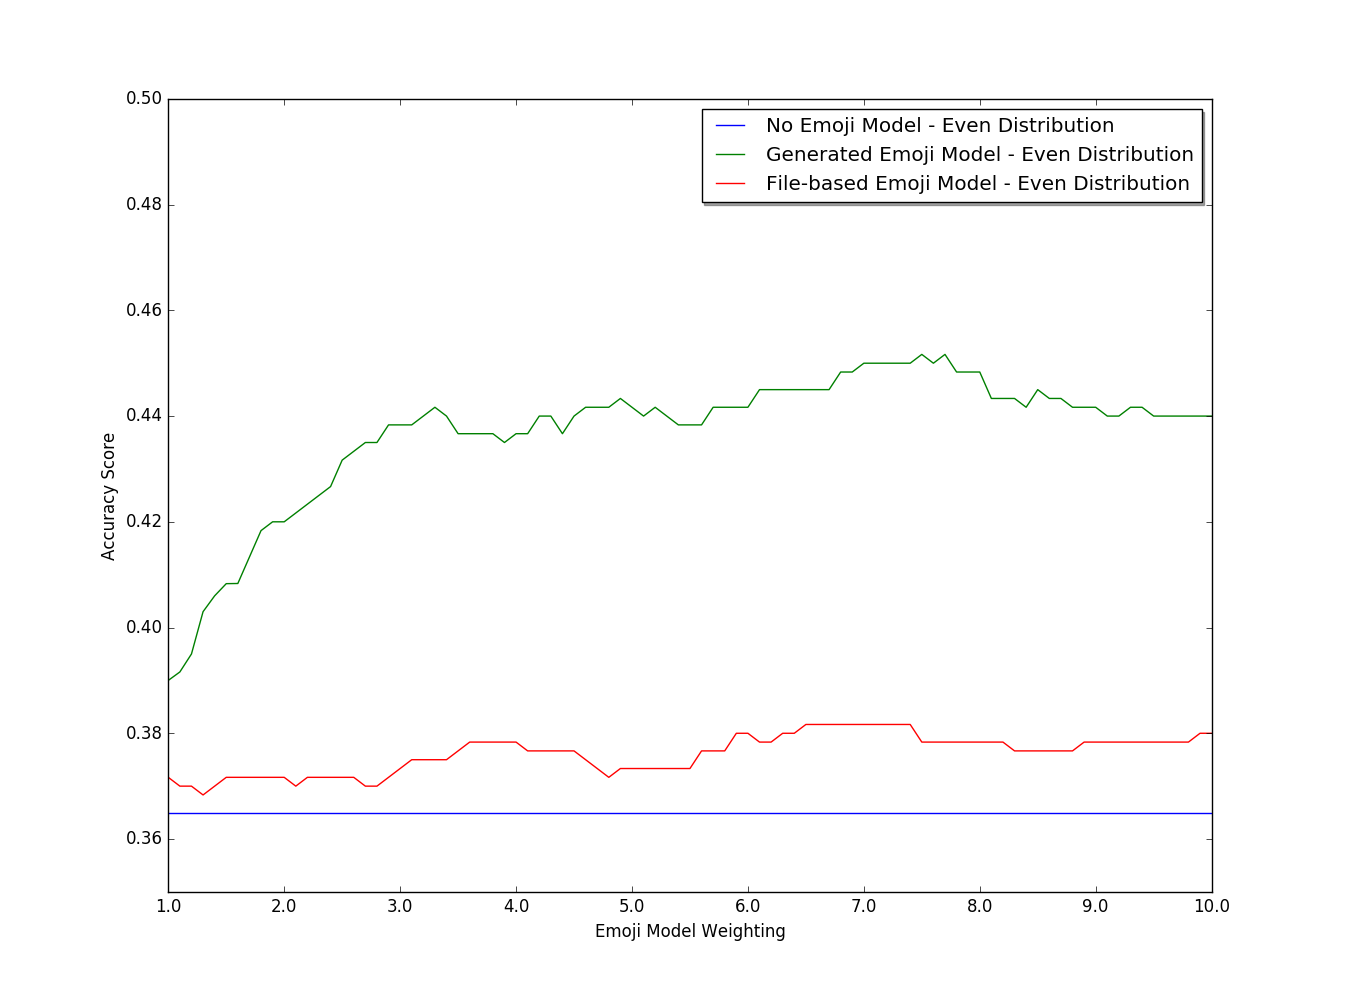
\includegraphics[width=13cm]{figures/emoji_models_even.png}
\caption{Accuracy of system over 600 emoji tweets (300 per emotion) when adjusting the emoji model weighting}
\end{figure}

The score when using no model does not change as the weighting has nothing to apply itself too.

The rule-based emoji look up method has a slight increase in accuracy. We peak with a score around 0.38 when using a weighting of 7.0. This is a 2\% increase over not applying an additional model to deal with the emojis.

Our generated model performs the best and presents an apparent growth in performance as we increase the model's weighting. We peak around \textbf{0.45} system accuracy; this is the highest score we have achieved so far when using an evenly distributed test set. This score also out-ranks the accuracy of using the old classifier with the old training data over an even distribution.
 
Applying our distributed emoji model is something we should certainly do. The system has nothing to lose, as tweets that do not contain any emojis will not be affected, but tweets that do include emojis have a better chance of being correctly classified.


\begin{equation}
\begin{split}
\hat{w} = \argmax_{e \in E} \\ 0.5 SM \sum_{t}^{T} \log P(t \mid e)  + \\ 1.0 DM \sum_{t}^{T} \log P(t \mid e) + \\  7.0 EM \sum_{e}^{E} \log Score(e)
\end{split}
\end{equation}

\begin{equation}
Score = \frac{Count (E_j,T_ej \in T)}{Count(T_ej \in T)}
\end{equation}

Where $E_j$ is a tweet that contains a \textit{given} emoji. $T$ is the whole set of tweets and  $T_ej$ is a tweet of a \textit{given} emotion that contains \textit{any} emoji.

% \chapter{Appendix 1} \label{app1}

\section{Comparing ngram size} \label{ngram}

Here we are comparing the average accuracy across 10 folds of using different ngram size ranges. We include two different classifiers.

\begin{figure}[H]
\center
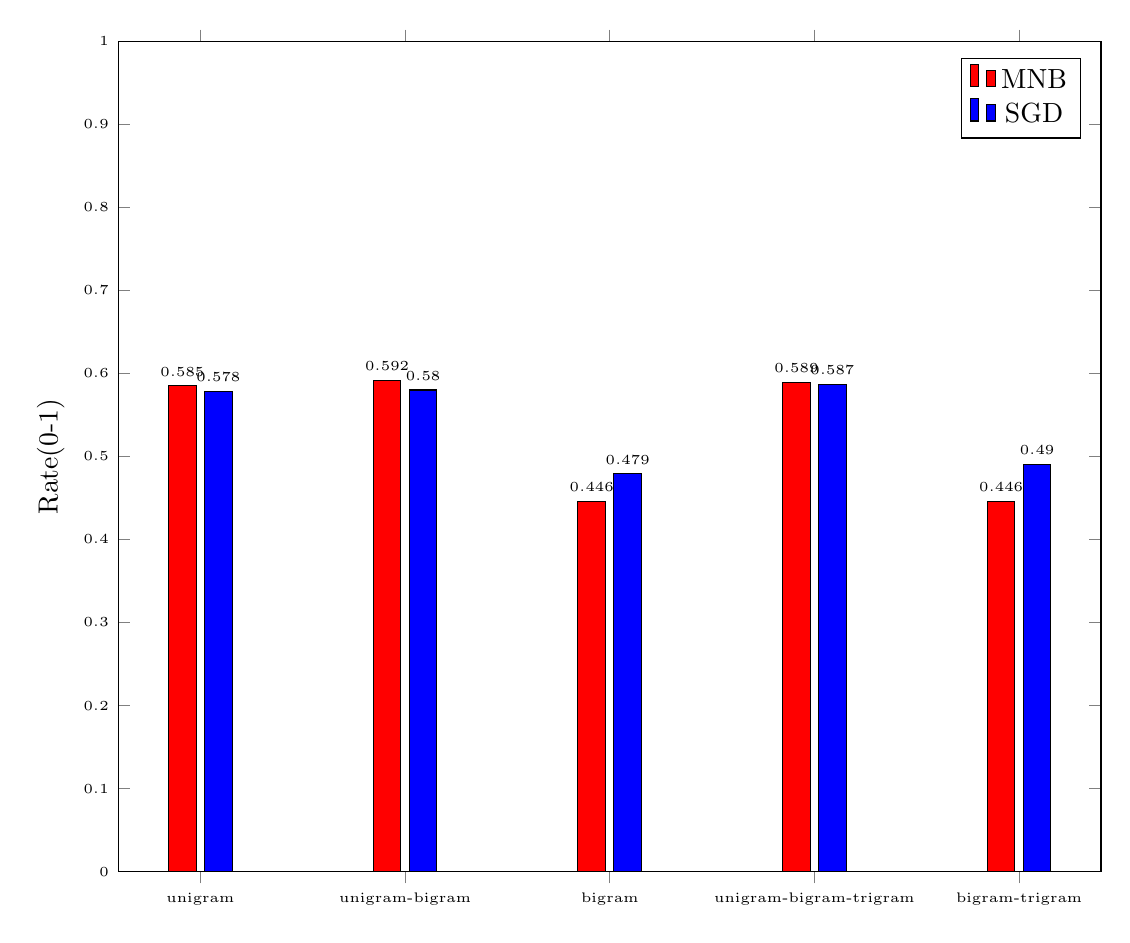
\begin{tikzpicture}
\begin{axis}[
	ymin = 0,
	ymax = 1,
	width = 400,
	symbolic x coords={unigram,unigram-bigram,bigram,unigram-bigram-trigram,bigram-trigram},
    xtick=data,
	ylabel=Rate(0-1),
	compat=newest, %Better label placement,
	ybar = 3,
	nodes near coords,
	scaled x ticks = false,
	tick label style={font=\tiny} ,
	every node near coord/.append style={/pgf/number format/fixed, /pgf/number format/precision=3, font=\fontsize{1}{1}\selectfont},
]


\addplot [ybar, fill=red]
	coordinates {
		(unigram,0.585) (unigram-bigram,0.592)
		 (bigram,0.446) (unigram-bigram-trigram,0.589) (bigram-trigram, 0.446)
		 
		 };
		 
		 
\addplot [ybar, fill=blue]
	coordinates {
		(unigram,0.578) (unigram-bigram,0.580)
		 (bigram,0.479) (unigram-bigram-trigram,0.587) (bigram-trigram, 0.490)
		 
		 };
		 
		 				 	
\addlegendentry{MNB}
\addlegendentry{SGD}
\title{F-Measure Rates}
\end{axis}
\end{tikzpicture}
\caption{Comparison of average accuracy between ngram ranges across 10 folds}
\end{figure}


\section{Comparing df} \label{df}

Here we are comparing minimum document frequency and the average system accuracy that results.

\begin{figure}[H]
\center
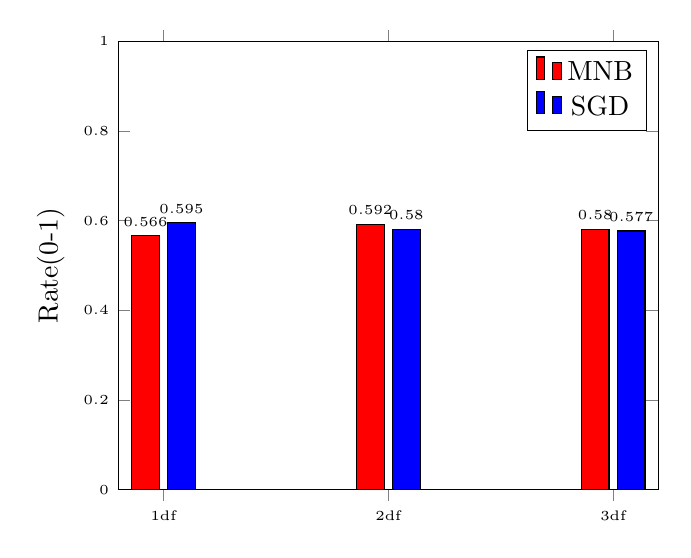
\begin{tikzpicture}
\begin{axis}[
	ymin = 0,
	ymax = 1,
	symbolic x coords={1df,2df,3df},
    xtick=data,
	ylabel=Rate(0-1),
	compat=newest, %Better label placement,
	ybar = 3,
	nodes near coords,
	scaled x ticks = false,
	tick label style={font=\tiny} ,
	every node near coord/.append style={/pgf/number format/fixed, /pgf/number format/precision=3, font=\fontsize{1}{1}\selectfont},
]


\addplot [ybar, fill=red]
	coordinates {
		(1df, 0.566) (2df,0.592)
		 (3df,0.580) 
		 
		 };
		  
\addplot [ybar, fill=blue]
	coordinates {
		(1df,0.595) (2df,0.580)
		 (3df,0.577)
		 
		 };
		 
		 				 	
\addlegendentry{MNB}
\addlegendentry{SGD}
\title{F-Measure Rates}
\end{axis}
\end{tikzpicture}
\caption{Comparison of average accuracy between df threshold across 10 folds}
\end{figure}


\section{Full Comparison of Stemmers and Lemmatizers} \label{comp_stem}

\begin{figure}[H]
\center
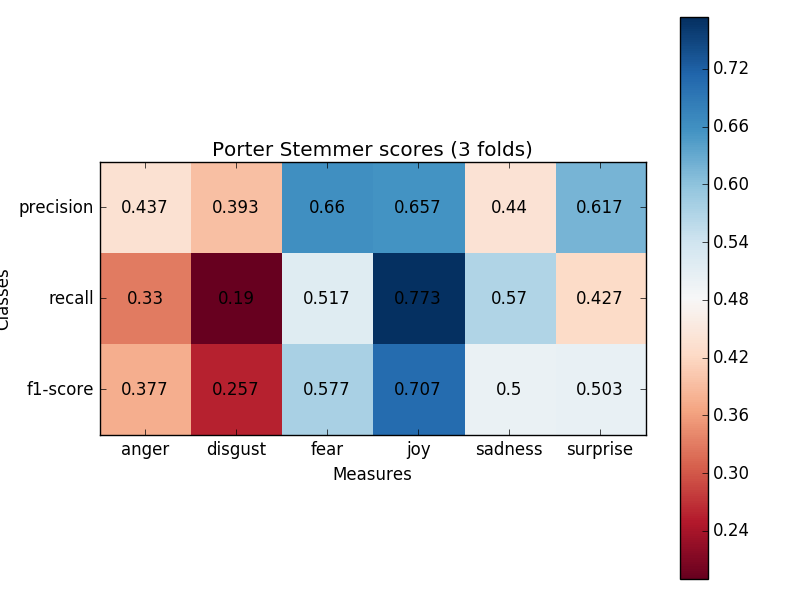
\includegraphics[width=12cm]{images/porter_matrix.png}
\caption{Confusion Matrix for Porter Stemmer}
\end{figure}


\begin{figure}[H]
\center
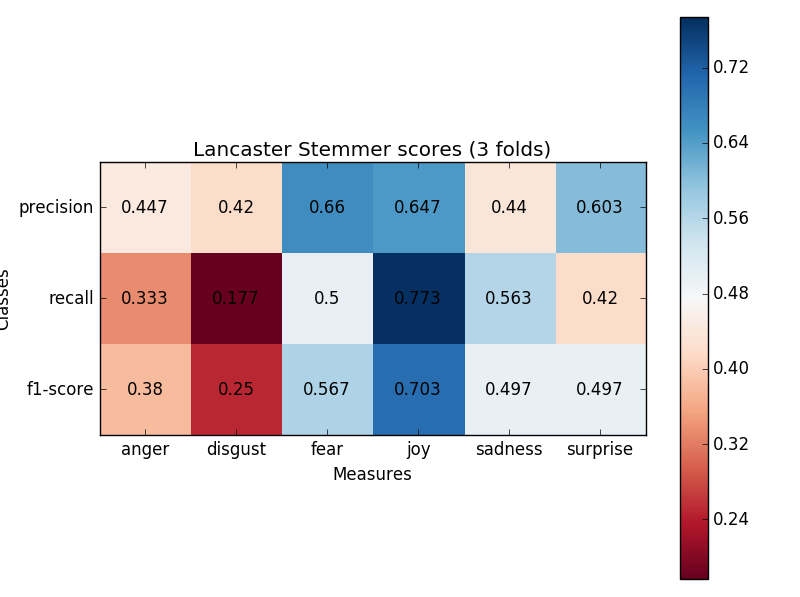
\includegraphics[width=12cm]{images/Lancaster_matrix.png}
\caption{Confusion Matrix for Lancaster Stemmer}
\end{figure}

\begin{figure}[H]
\center
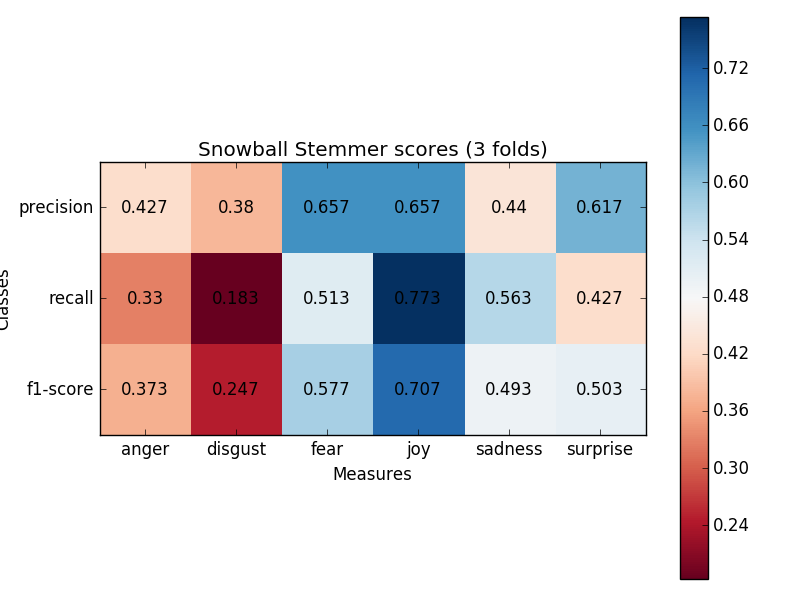
\includegraphics[width=12cm]{images/Snowball_matrix.png}
\caption{Confusion Matrix for Snowball Stemmer}
\end{figure}

\begin{figure}[H]
\center
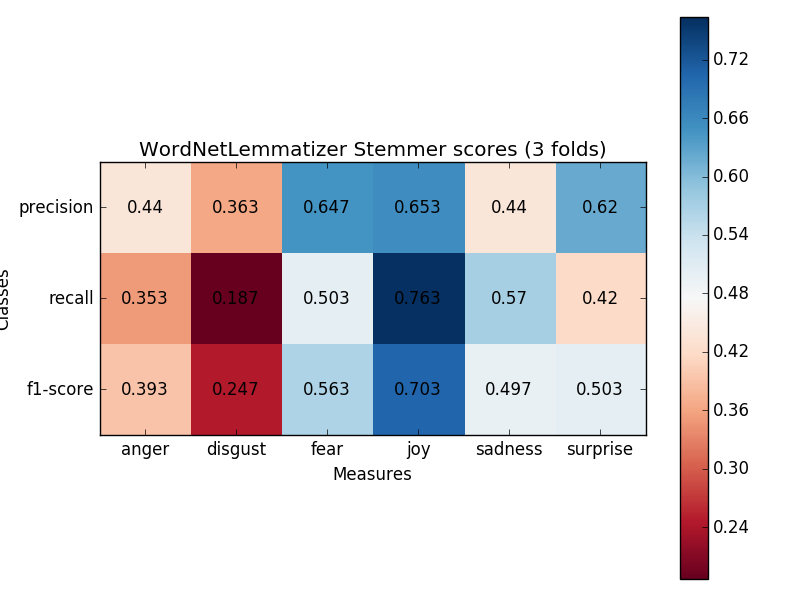
\includegraphics[width=12cm]{images/WordNetLemmatizer_matrix.png}
\caption{Confusion Matrix for WordNetLemmatizer}
\end{figure}

\bibliographystyle{acm} 
\bibliography{mybibliography} 


\end{document}
